
%%%%%%%%%%%%%%%%%%%%%%%%%%%%%%%%%%%%%%%%%%%%%%%%%%%%%%%%%%%%%%%%%%
%%%%%%%% ICML 2012 EXAMPLE LATEX SUBMISSION FILE %%%%%%%%%%%%%%%%%
%%%%%%%%%%%%%%%%%%%%%%%%%%%%%%%%%%%%%%%%%%%%%%%%%%%%%%%%%%%%%%%%%%

% Use the following line _only_ if you're still using LaTeX 2.09.
%\documentstyle[icml2012,epsf,natbib]{article}
% If you rely on Latex2e packages, like most moden people use this:
\documentclass{article}

% For figures
\usepackage{graphicx} % more modern
%\usepackage{epsfig} % less modern
\usepackage{subfigure} 

% For citations
\usepackage{natbib}

% For algorithms
\usepackage{algorithm}
\usepackage{algorithmic}

% As of 2011, we use the hyperref package to produce hyperlinks in the
% resulting PDF.  If this breaks your system, please commend out the
% following usepackage line and replace \usepackage{icml2012} with
% \usepackage[nohyperref]{icml2012} above.
\usepackage{hyperref}

% Packages hyperref and algorithmic misbehave sometimes.  We can fix
% this with the following command.
\newcommand{\theHalgorithm}{\arabic{algorithm}}

% Employ the following version of the ``usepackage'' statement for
% submitting the draft version of the paper for review.  This will set
% the note in the first column to ``Under review.  Do not distribute.''
%\usepackage{icml2012} 
% Employ this version of the ``usepackage'' statement after the paper has
% been accepted, when creating the final version.  This will set the
% note in the first column to ``Appearing in''
\usepackage[accepted]{icml2012}

%-------
\usepackage{times}
\usepackage{epsfig}
\usepackage{graphicx}
\usepackage{amsmath}
\usepackage{amssymb}
\usepackage{subfigure}
\usepackage{cancel}
\usepackage{color}
\usepackage{hyperref}
%\usepackage{multicol}
%\usepackage{blindtext}

%\usepackage[usenames,dvipsnames]{color}

\newcommand{\highlight}[1]{\colorbox{yellow}{#1}}
\newcommand{\bff}{\mathbf{f}}
\newcommand{\bfu}{\mathbf{u}}
\newcommand{\bfy}{\mathbf{y}}
\newcommand{\bfx}{\mathbf{x}}
\newcommand{\bft}{\mathbf{t}}
\newcommand{\bfk}{\mathbf{k}}
\newcommand{\bfzi}{\mathbf{z}}
\newcommand{\bfw}{\mathbf{w}}
\newcommand{\bfmu}{\boldsymbol \mu}
\newcommand{\bfz}{\mathbf{0}}
\newcommand{\bftheta}{\boldsymbol \theta}
\newcommand{\T}{{\top}}
\newcommand{\bfa}{\mathbf{a}}
\newcommand{\bb}{\beta^{-1}}
\newcommand{\la}{\left\langle}
\newcommand{\ra}{\right\rangle}
\newcommand{\vv}{\vartheta}
\newcommand{\intd}{\text{d}}
\newcommand{\ie}{i.e.\ }
\newcommand{\eg}{e.g.\ }

%------------
\definecolor{light-gray}{gray}{0.43}



% The \icmltitle you define below is probably too long as a header.
% Therefore, a short form for the running title is supplied here:
\icmltitlerunning{Manifold Relevance Determination}


\begin{document}

\twocolumn[
\icmltitle{Manifold Relevance Determination}

% It is OKAY to include author information, even for blind
% submissions: the style file will automatically remove it for you
% unless you've provided the [accepted] option to the icml2012
% package.
%\icmlauthor{Andreas C. Damianou$^1$}{Andreas.Damianou@sheffield.ac.uk} \\
%%\icmladdress{Dept. of Computer Science \& Sheffield Institute for Translational Neuroscience, University of Sheffield, UK}
%\icmlauthor{Carl Henrik Ek}{chek@csc.kth.se}
%\icmladdress{KTH -- Royal Institute of Technology, CVAP Lab, Stockholm, Sweden}
%\icmlauthor{Michalis K. Titsias}{mtitsias@well.ox.ac.uk}
%\icmladdress{Wellcome Trust Centre for Human Genetics, Roosevelt Drive, Oxford OX3 7BN, UK }
%\icmlauthor{Neil D. Lawrence$^2$}{n.lawrence@sheffield.ac.uk}
%\icmladdress{$^{1,2}$Dept. of Computer Science \& Sheffield Institute for Translational Neuroscience, University of Sheffield, UK}

\icmlauthor{Andreas C. Damianou}{Andreas.Damianou@sheffield.ac.uk}
\icmladdress{Dept. of Computer Science \& Sheffield Institute for Translational Neuroscience, University of Sheffield, UK}
\icmlauthor{Carl Henrik Ek}{chek@csc.kth.se}
\icmladdress{KTH -- Royal Institute of Technology, CVAP Lab, Stockholm, Sweden}
\icmlauthor{Michalis K. Titsias}{mtitsias@well.ox.ac.uk}
\icmladdress{Wellcome Trust Centre for Human Genetics, Roosevelt Drive, Oxford OX3 7BN, UK }
\icmlauthor{Neil D. Lawrence}{n.lawrence@sheffield.ac.uk}
\icmladdress{Dept. of Computer Science \& Sheffield Institute for Translational Neuroscience, University of Sheffield, UK}

% You may provide any keywords that you 
% find helpful for describing your paper; these are used to populate 
% the "keywords" metadata in the PDF but will not be shown in the document
\icmlkeywords{GP-LVM, Bayesian, machine learning, ICML}

\vskip 0.3in
]

% \begin{abstract} 
%   In this paper we present a fully Bayesian latent variable model
%   which exploits conditional non-linear (in)-dependence structures to
%   learn an efficient latent representation. The model is capable of
%   learning from extremely high-dimensional data such as directly
%   modelling high resolution images. The latent representation is
%   factorized to represent shared and private information from multiple
%   views of the data. Bayesian techniques allow us to automatically
%   estimate the dimensionality of the latent spaces. We demonstrate the
%   model by prediction of human pose in an ambiguous setting. Our
%   Bayesian representation allows us to perform disambiguation in a
%   principled manner by including priors which incorporate the dynamic
%   structure of the data. 
%   We demonstrate the ability of the model to
%   capture structure underlying extremely high dimensional spaces by
%   learning a low-dimensional representation of a set of facial images
%   under different illumination conditions. The model correctly
%   automatically creates a factorized representation where the lighting
%   variance is represented in a separate latent space from the variance
%   associated with different faces. We show that the model is capable
%   of generating morphed faces and images from novel light directions.
% \end{abstract} 

\begin{abstract} 
  In this paper we present a fully Bayesian latent variable model
  which exploits conditional non-linear (in)-dependence structures to
  learn an efficient latent representation. 
  The latent space is factorized to represent shared and private information from multiple
  views of the data. In contrast to previous approaches, we introduce a relaxation to
  the discrete segmentation and allow for a ``softly'' shared latent space.
  Further, Bayesian techniques allow us to automatically
  estimate the dimensionality of the latent spaces.
%
%   The model is capable of
%    capturing structure underlying extremely high dimensional spaces.
%   This is illustrated by directly modelling the pixels of a set of high resolution facial images
%   under different illumination conditions. We show that the model automatically
%   correctly separates the lighting variance from the one associated with different
%   face characteristics and is also able of generating morphed faces and images from novel light directions.
 The model is capable of capturing structure underlying extremely high dimensional spaces.
 This is illustrated by 
% directly modelling relatively large 
 modelling unprocessed images with tenths of thousands of pixels. This also allows us
 to directly generate novel images from the trained model by sampling from the discovered latent spaces.
%
  We also demonstrate the
  model by prediction of human pose in an ambiguous setting. Our
  Bayesian framework allows us to perform disambiguation in a
  principled manner by including latent space priors which incorporate the dynamic
  nature of the data. 
\end{abstract} 




%%%%%%%%% BODY TEXT
\section{Introduction}
%% Observations in Computer Vision are often extremely
%% high-dimensional. However, the dimensionality of the representation typically
%% does not reflect the intrinsic dimensionality of the data but is rather an effect of
%% the system that has acquired it. A central problem is finding
%% a new more efficient representation in order to circumvent
%% the \emph{curse of dimensionality} \cite{bellman1957dynamic}. Given a
%% set of data, a large range of dimensionality reduction approaches have
%% been suggested ranging from spectral methods, often based on
%% Multi-Dimensional Scaling \cite{Cox:2008uv}, to generative methods such
%% as GTM \cite{Bishop:1998fl}. The generative approaches build models
%% of the data and are in general founded on more sound principles, making
%% less restrictive assumptions about the data \cite{Ek:2009vv}. The
%% benefit of spectral methods is that they are 
%% convex and can be more efficient at handling large datasets.
%generally more efficient 
%in
%capable of
% handling large amounts of data in high dimensions.

Multiview learning is characterised by data which contain
observations from several different modalities: for example depth
cameras provide colour and depth images from the same scene, or a
meeting might be represented by both an audio and a video feed. This
motivates latent variable models which align the different views by
assuming that a portion of the data variance is shared between the
modalities, whilst explaining the remaining variance with latent
spaces that are private to each modality.  This model structure allows
inference when only a subset of the modalities is available and,
because the observation spaces have been aligned, it is possible to
transfer information between modalities by conditioning the model
through the underlying concept.

Several approaches that combine multiple views have been suggested.
One line of work aims to find a low-dimensional representation of the
observations by seeking a transformation of each view. Different
approaches exploit different characteristics of the data such as,
correlation \cite{Kuss:2003wp,Ham:2005vs}, or mutual information
\cite{Memisevic:2011tq}. However, these methods only aim to encode the
shared variance and do not provide a probabilistic model. To address
these shortcomings different generative models have been suggested.
In particular, approaches formulated as Gaussian Processes Latent
Variable Models (GP-LVMs) \cite{Lawrence:2005vk} have been especially
successful \cite{Shon:2006wr,Ek:2007uo}. However, these models assume
that a single latent variable is capable of representing each
modality, implying that the modalities can be fully aligned.  To
overcome this, the idea of a factorized latent space was presented in
\cite{Ek:2008up} where each view is associated with an additional
\emph{private} space, representing the variance which cannot be
aligned, in addition to the shared space \cite{Ek:2009vv}, an idea
independently suggested by \citet{Klami06mlsp}.  The main challenge for the
applicability of the proposed models is that the factorization of the
latent variable is a structural and essentially discrete property of
the model, making it very challenging to
learn. \citet{Salzmann:2010vh} introduced a set of regularizers
allowing the dimensionality of the factorization to be learned.
However, the regularizers were motivated out of necessity rather than
principle and introduced several additional parameters to the model.

We present a new principled approach to learning a factorized latent
variable representation of multiple observation spaces. We introduce a
relaxation of the structural factorization of the model from the
original \emph{hard} discrete representation, where each latent
variable is either associated with a private space or a shared space,
to a smooth continuous representation, where a latent variable may be
more important to the shared space than the private space. In contrast
to previous approaches the model is fully Bayesian, allowing
estimation of both the dimensionality and the structure of the latent
representation to be done automatically. Further, it provides an approximation to the full posterior of the latent points given the data.% distribution.
 We describe the model and the
variational approximation in the next section. The model is capable of
handling extremely high dimensional data. We illustrate this by
modelling image data directly in the pixel space in section
\ref{experiments}. We also demonstrate the model's ability to reconstruct pose from silhouette in a human motion example and, finally, by considering class labels to be a second `view' of a dataset we show how the model can be used to improve classification performance in a well known visualization benchmark: the ``oil data''.

% The remainder of the paper is structured as follows: section
% \ref{model} details the proposed model and section 
% describes experiments conducted on high dimensional image data, on a
% multi-modal human pose dataset and on a classification task. Based on
% the results and the analysis performed there, we present our final
% conclusions in section
% \ref{conclusions}.


%%% Local Variables: 
%%% mode: latex
%%% TeX-master: "../svargplvmICML2012"
%%% End: 


\section{The Model \label{model}}
Given two separate datasets $Y \in \mathbb{R}^{N\times D_Y}$ and
$Z\in\mathbb{R}^{N\times D_Z}$ we seek a parametrization within the
same model. Specifically, we assume the existence of a single
low-dimensional latent variable $X\in \mathbb{R}^{N\times Q}$ which
through the mappings $f_Y: X \mapsto Y$ and $f_Z: X \mapsto Z$ is
capable of representing the high dimensional data. 
Assuming the observed
data to have been corrupted by additive Gaussian noise,
\begin{align}
  \mathbf{y}_n &= f_Y(\mathbf{x}_n) + \epsilon_n\nonumber\\
  \mathbf{z}_n &= f_Z(\mathbf{x}_n) + \epsilon_n,
\end{align}
we can formulate the likelihood of the data under the model,
$P(Y,Z|X,\bftheta)$ where $\bftheta$ are the parameters of the generating
mappings. Finding the latent representation $X$ and the mappings $f_Y$
and $f_Z$ is a very ill-constrained problem with an infinite number of
possible solutions. To provide intuition, one analogy would be to think
of meeting a friend in a bar, clearly a nearly infinite number of combinations
of starting positions and paths exist for your friend to end up at
just this specific bar at this time. Being your good friend, you
probably have a reasonably good idea about his whereabouts and habits
so from this information you would be able to limit the number of
possibilities. Very much similar to this analogy, the way to proceed
here is to exploit priors to regularize the problem.

A very successful approach in dimensionality reduction has been regularizing the
 problem by placing Gaussian Processes
\cite{Rasmussen:book06} priors over the generating mapping as
introduced by \cite{Lawrence:2005vk}, and referred to as a Gaussian Process
Latent Variable Model (GP-LVM). The use of such priors has also been
exploited when multiple observation spaces are available, as in
\cite{Shon:2006wr,Ek:2007uo}. However, these approaches used a maximum a posteriori (MAP)
solution which rendered them challenging to learn and significantly
reduced their flexibility. A specific problem associated with these methods is that
they introduced the assumption that all variance in the observed data that
was not shared had to be explained away as spherical Gaussian noise, since it was not
possible to learn the observation space's specific relevance of each
latent dimension.

To circumvent these problems our model makes use of the
variational Bayesian framework and its dynamical extension as recently
proposed by Titsias and Lawrence \cite{Titsias:bayesGPLVM10}, and
Damianou \textit{et al.}  \cite{Damianou:vgpds11} respectively.
They show that a prior distribution $p(X)$ can be placed over
the latent space which can then be approximately marginalised out, so
that the objective function used in the training procedure is no
longer conditioned on $X$. This allows for \emph{Automatic Relevance
  Determination (ARD)} priors \cite{Rasmussen:book06} to be used for
the mappings, so that a set of weights defines the ``importance'' of
each latent dimension. This means that we can learn a ``soft''
factorization of the latent space without having to rely on hand crafted
regularizers such as in \cite{Salzmann:2010vh}.

\par In our method, we use ARD GP priors for our
mappings $f_Y$ and $f_Z$. In this way, we can learn a common latent
space\footnote{Actually we learn a common \emph{distribution} of
  latent points, giving us a set of latent points (mean of the
  distribution) and associated variance.} but we allow the two sets of
ARD weights, $\bfw_Y = \{ w^{(q)}_Y \}_{q=1}^Q$ and $\bfw_Z = \{
w^{(q)}_Z \}_{q=1}^Q$ to automatically infer the responsibility of
each latent dimension for generating points in the $Y$ and $Z$ spaces
respectively.  We can then automatically recover a segmentation of the
latent space $X = \left( X_Y, X_s, X_Z \right)$, where $X_s \in
\mathbb{R}^{N \times Q_s}$ is the shared subspace, defined by the set
of dimensions $q \in [1, ... ,Q]$ for which $w_Y^{(q)}, w_Z^{(q)} >
\epsilon$, with $\epsilon$ being a number close to zero. This equips
the model with further flexibility, because
it allows for a ``softly'' shared latent space, if the two sets of weights are
both greater than $\epsilon$ but dissimilar, in general.  As for the
two private spaces, $X_Y$ and $X_Z$, their dimensionalities $Q_Y$ and
$Q_Z$ are also being inferred automatically.  More precisely:
\begin{equation}
X_Y = \{ \bfx_q \}_{q=1}^{Q_Y}: \bfx_q \in X, \; w_Y^{(q)} > \epsilon, \;  w_Z^{(q)} < \epsilon
\end{equation}
and analogously for $X_Z$. Here, $\bfx_q$ denotes columns of $X$, while we assume that
data are stored by rows.
 Notice that, in general, there will also be
dimensions of the initial latent space which are considered
unnecessary by both sets of weights. If the subspace corresponding to
these irrelevant latent dimensions is denoted with $X_U$, then the actual factorisation
can be written more precisely as $X = \left( X_Y, X_s, X_Z, X_U
\right)$.  All of the above are summarised in graphical model
\ref{fig:grModel}.

%
%\subsection{GP-LVM-based models}
%
%The Gaussian Process Latent Variable Model \cite{Lawrence:2005vk} (GPLVM) is a fully probabilistic, latent variable
% model which enables nonlinear dimensionality reduction and can be seen, therefore, as a more powerful generalisation of
% PPCA. 
%GP-LVM is generative and assumes that the observed $N$ $D$-dimensional datapoints, collectively represented as
% $Y \in \mathbb{R}^{N \times D}$, are generated by a lower dimensional space
% $X \in \mathbb{R}^{N \times Q}$ ($Q \ll D$) via a mapping $f$:
%\begin{equation}
%\label{generative}
%y_{nd} = f_d(\bfx_n) + \epsilon_{nd}, \;\; \epsilon_{nd} \sim \mathcal{N}(0, \beta^{-1}).
%\end{equation}
%Here, $y_{nd}$ denotes the element from the $n$th row and $d$th column of $Y$ and $\epsilon_n$ is a Gaussian noise term.
% Further, we use the notation
%$\bfx_n$ and $\bfy_n$ to refer to rows from $X$ and $Y$ respectively and $x_q$, $y_d$ to refer to columns of these matrices.
%
%The mapping from the latent to the observed space is learned by a product of Gaussian processes which act as a prior.
%%:
%%\begin{equation}
%%\label{gppriorf}
%%f_d(\bfx)  \sim  \mathcal{GP}(0, k_f(\bfx_i,\bfx_j)), \ \ d=1,\ldots,D.
%%\end{equation}
%%where $k_f(\bfx_i,\bfx_j)$ is the covariance function of the GPs, parametrised by a vector of parameters $\bftheta_f$.
%
%\par The standard GP-LVM model defined above, is trained by optimising the likelihood
% $p(Y|X,\bftheta)$, which acts as an objective function. In that way, MAP estimates are found for the model
% parameters $\bftheta$ and the set of latent points $X$. However, conditioning the objective function on $X$ means
% that the number of latent dimensions $Q$ has to be set by hand, or selected non-automatically after exhaustive model selection.
%
%\noindent  \\
%\noindent  \\
%
% \par \textbf{NOTES on the rest}: \\
%\par \textcolor{red}{* 2-3 lines about Bayesian GPLVM and dynamical extension, and the definition of the variational bound
%(which equivalently to the likelihood is the objective function) as $\mathcal{L}(Y) + \text{KL(q(X)||p(X)}$, where the first includes
%the data and the second only the prior, with the link being done by a variational distribution $q(X)$}
%
%\noindent  \\
%
%\subsection{Subspace model}
%
%
%\par \textcolor{red}{* Exploit the fact that the prior and the data exist in different terms, so that we can define a subspace model
%with objective function $\mathcal{L}(Y_1) + \mathcal{L}(Y_2) + ... + \mathcal{L}(Y_M) + \text{KL}(q(X)||p(X)$. 
%Then, $X$ can be shared but thanks to the Bayesian training, the ARD parameters of the cov. function can select subsets of the
%whole $X$. By keeping the sub-models separate and only linking them via the obj. function, we know which model (\ie which dataset $Y_m$)
%selected which subspace of $X$.}
%
%\noindent \\
%
%\par \textcolor{red}{* Or, we can start defining directly the shared model and then explaining GP-LVM and Bayesian GP-LVM on the way...}

\begin{figure*}
  \begin{center}
    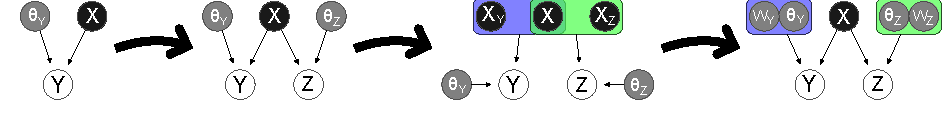
\includegraphics[width=0.9\textwidth]{bin/graphicalmodel.pdf}
  \end{center}
  \vspace{-8pt}
  \caption{\small {\it The above figure shows the evolution of the
      topology of the GP-LVM model chronologically from left to
      right. On the far left the original model is shown, where a
      single latent variable $X$ is used to represent the
      observed data $Y$. From the original model a range of
      different models for the shared data scenario have been
      proposed. The first model made an assumption that all of the
      variance in the observations was shared. This meant that the
      model was applicable to scenarios where the aim was to align two
      different manifolds. To overcome this problem a model with
      private space was introduced. However, this factorization
      introduced further challenges when learning the model. The right
      most image shows the model we propose in this paper. By
      introducing additional hyperparameters to the model encoding the
      relevance of each dimension independently for the observation
      spaces we can automatically learn the factorization of the data.
  }}
 \label{fig:grModel}
\end{figure*}

%% \begin{figure}[ht]
%% \begin{center}
%%   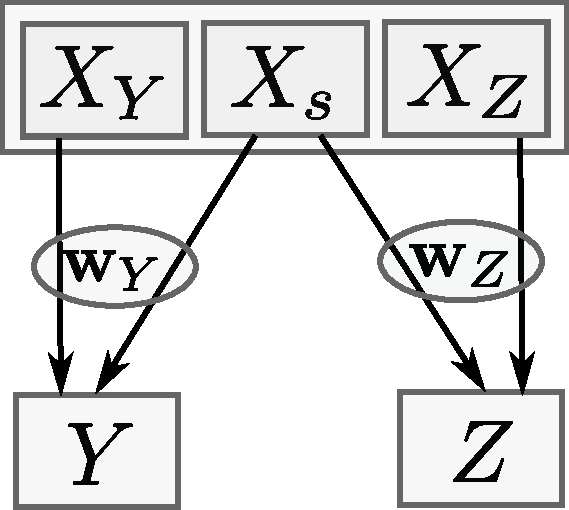
\includegraphics[width=0.18\textwidth]{../diagrams/grModel}
%% \end{center}
%% \vspace{-9pt}
%% \caption{\small{
%% .....}}
%% \label{fig:grModel}
%% \end{figure}

\par The fully Bayesian training procedure requires maximisation of
the logarithm of the joint
\emph{marginal} likelihood $p(Y,Z | \bftheta)$, where $\bftheta$ is the set of model parameters.
Although this quantity is intractable, we can invoke the variational framework of 
\cite{Titsias:bayesGPLVM10,Damianou:vgpds11} and
approximate it with a variational lower bound $\mathcal{F}_v(q,\bftheta) \approx p(Y,Z | \bftheta)$
 which relies on a variational
distribution $q(X)$. This distribution is defined in the same manner as in the \cite{Titsias:bayesGPLVM10,Damianou:vgpds11},
where it is also shown that for a single output space $Y$, the variational lower bound
breaks into two terms 
$\mathcal{L}(Y) + \text{KL}\left[ q(X) || p(X) \right]$, where the first contains
the data $Y$ and the second only involves the prior on $X$. The variational distribution $q(X)$
``binds'' the two terms together. Exploiting this observation for our model, which jointly learns
a common (factorised) latent space, allows us to write:
\begin{equation}
\mathcal{F}_v(q,\bftheta) = \mathcal{L}(Y) + \mathcal{L}(Z) + \text{KL} \left[ q(X) || p(X) \right],
\label{eq:bound}
\end{equation}
which is trivially extended for more than two observed datasets. This is
our final objective function, which is jointly maximised with respect to the model parameters (involving
the mapping parameters for $f_Y$ and $f_Z$ and the corresponding weights $\bfw_Y$ and $\bfw_Z$) and
the variational parameters.

All of the involved terms on the r.h.s of \eqref{eq:bound} are computed exactly as described in \cite{Titsias:bayesGPLVM10,Damianou:vgpds11}.
This means that, as observed in \cite{Damianou:vgpds11}, the data are only involved
in the quantities $Y Y^\T$ and $Z Z^\T$ which are $N \times N$ matrices no matter how many features
$D_Y$ and $D_Z$ are used to describe the original data. Also, these quantities are constant and can
be precomputed. Consequently, our approach is able to model datasets with millions of features.

Further, analogously to \cite{Titsias:bayesGPLVM10,Damianou:vgpds11}, the optimisation procedure simultaneously allows
the variational distribution $q(X)$ to approximate the true posterior $p(X|Y,Z)$, \ie we obtain a distribution
over the latent space. This adds extra robustness to our model, since previous approaches rely on
MAP estimates for the latent points.

%Unlike previous MAP methods, we train our model by using an approximation to the logarithm of
%the joint \textit{marginal} likelihood $\mathcal{F}_v(q, \bftheta) \approx p(Y,Z | \bftheta)$ as an objective function, where
%$\bftheta$ is the set of all model parameters and $q$ refers to the variational distribution
%which renders the approximation tractable. . We exploit the fact that in the variational
%Bayesian framework of \cite{Titsias09} the marginal likelihood $p(Y)$ of a single dataset $Y$
%breaks into two different terms 
%.... \textcolor{red}{bound, training etc.}

%$\mathcal{L}(Y) + \text{KL(q(X)||p(X)}$, where the first includes
%the data and the second only the prior, with the link being done by a variational distribution $q(X)$}

% As shown in \cite{Titsias09}, the variatio
\subsection{Dynamical Modelling}

The model formulation described in the previous section is also covering the case
when we wish to additionally model correlations between datapoints of the same output space, \ie when
$Y$ and $Z$ are multivariate timeseries. For the dynamical scenario
we follow \cite{Damianou:vgpds11,Lawrence:hgplvm07} and choose the prior on the
 latent space to depend on the times 
$\bft \in \mathbb{R}^N$ when the observations were made. In terms of computations, this
 only affects the KL term of equation \eqref{eq:bound}, which can be calculated as described
 in \cite{Damianou:vgpds11}. With this approach, we are also allowed to 
% efficiently model multiple independent sequences which, nevertheless share some commonality. 
learn the structure of multiple correlated sequences.
This is done by learning a common latent space for all timeseries while, at the same time, ignoring
correlations between datapoints that belong to different sequences.



\subsection{Inference \label{inference}}

Given a model which is trained so as to jointly represent two output spaces $Y$ and $Z$ with
a common, but factorised input space $X$, we wish to generate a new (or infer a training) set of outputs
$Z^* \in \mathbb{R}^{N^* \times D_Z}$ given a set of (potentially partially) observed test points $Y^* \in \mathbb{R}^{N^* \times D_Y}$.
This is done in three steps. Firstly, we predict the set of latent points $X^* \in \mathbb{R}^{N^* \times Q}$
which is most likely to have generated $Y^*$. For this, we use an approximation to the posterior $p(X^*|Y^*,Y)$
as is done for the standard Bayesian GP-LVM model \cite{Titsias:bayesGPLVM10,Damianou:vgpds11} and is
similar to the variational distribution $q(X)$ learned during training.
In the second step, we find the training latent points $X_{NN}$ which are closest to $X^*$ in the \emph{shared}
latent space. 
In the third step, we find outputs $Z$ from the GP-LVM likelihood $p(Z | X_{NN})$.

\par This procedure returns the set of training points $Z$ which best match the observed test points $Y^*$.
To generate novel outputs, we have to propagate the information recovered when predicting $X^*$. 
A simple way of doing this is to replace the features of $X_{NN}$ corresponding to the shared latent space,
 with those of $X^*$. This is a reasonable idea, since the shared latent space is supposed to encode the same
 kind of information for both datasets.
 A slightly more sophisticated approach is to also exploit the continuous nature of the
 optimised weights $\bfw_Y$ and give less importance to the dimensions of $X^*$ for which $w_Y^q$ is small,
 because these features are predicted with large uncertainty (variance).
 For example, we can create a new set of latent points $\hat{X}^{*}$ so that its private dimensions match those
 of $X_{NN}$ and its shared dimensions are found by averaging  
the shared dimensions of $X^*$ and $X_{NN}$ 
 as appropriate based on $\bfw_Y$. We can then generate outputs from $p(Z^* | \hat{X}^{*})$.

%We use $C_s$ to refer to the set of indices associated with the dimensions of the latent shared subspace,
%\ie $X_s = \{ \bfx_q\}_{q \in C_s}$.
%\begin{algorithm}
%\caption{Inference for SBGPLVM}
%\label{inferenceAlgorithm}
%\begin{algorithmic}
%\STATE \textbf{Input:} $Y^* = [ \bfy_1^*, ... , \bfy_N^* ], \bfy_n^* \in \mathbb{R}^{D_Y}$
%\STATE ...
%%\REPEAT
%	%\STATE $\forall q$ find $\mathit{S_q^{(k)}}$ from equation \eqref{SFixedPointQ} with $\tilde{\boldsymbol \theta}^{(k-1)}$ being fixed.
%	%\STATE Use a gradient-based method to find
%	%    $\underset{\tilde{\boldsymbol \theta}^{(k)}}{\operatorname{max}} \mathit{F(q, \boldsymbol \theta)}$ 
%	%    from equation \eqref{boundFinal} with $\mathit{S}^{(k)}$ fixed.
%    %\STATE $k = k+1$
%%\UNTIL{convergence}
%\end{algorithmic}
%\end{algorithm}


\section{Experiments \label{experiments}}
The goal of our method is to learn the shared and private spaces of distinct datasets which, nevertheless, have some underlying commonality.
For this reason, for each experiment we consider \emph{pairs} of (possibly heterogeneous) datasets, although the model can as well be applied
to more than two subsets.
The two pairs of datasets considered here are different in nature, allowing us to explore the various properties of our method. 
%
%Firstly,
%we consider a set of very high dimensional images belonging two six different human faces, spread into two datasets. The principal underlying
%commonality of the two subsets, which our method effectively discovers, is the varying light condition of the images. As a second
%experiment, we opted for a set of recordings of various human motions which is provided in two different representations: a subset containing %pose data and a subset containing the
%the corresponding silhouette features. 
%
The performance of the model is evaluated in different tasks, such as visualisation and interpretation
of the latent space which is discovered and segmented automatically, correspondence of datapoints between the two subsets of the given
datasets, as well as generation of new data.

Source code for recreating these experiments is included as supplementary material.

\subsection{Yale faces dataset}
The Yale dataset \cite{YaleFaces1, YaleFaces2} contains images of several human faces under different poses and 64 illumination conditions.
Here we consider only one pose, so that the images of a single subject differ only in the location of the light source.
As the images are high dimensional ($192 \times 168 = 32,256$ pixels), a common tactic is to rescale or preprocess them
 to extract fewer but more informative features. However, in our experiments we work directly
with the full set of raw pixel values to demonstrate the ability of our method to model data with a very large number of features. 
With this approach, we can also directly sample new images from the learned model.

\subsubsection{Modeling one face}

Before we proceed to subspace modelling, we first fit the standard Bayesian GP-LVM model to the whole set of $64$ images belonging to a single face, to visualise and assess the quality of the discovered latent space.
The model was initialised with $Q=15$ latent dimensions, and the Bayesian training not only discovered the effective dimensionality of the latent space automatically,
but it also defined the ``importance'' of each dimension. As can be seen in figure \ref{fig:yaleOneFaceScales}, most of the mapping kernel's weights were driven close to zero, signifying that the 
latent space is dominated by the three dimensions which have been assigned large weights.

In figures
\ref{fig:yaleOneFaceX21} and \ref{fig:yaleOneFaceX23}, one can see that the projection of the latent space into the 3 most dominant dimensions is shaped as a hollow 
hemishpere, which is in accordance with the shape of the space defined by the fixed locations of the light source.

\hspace{-6pt}
\begin{figure}[ht]
\begin{center}
\subfigure[]{
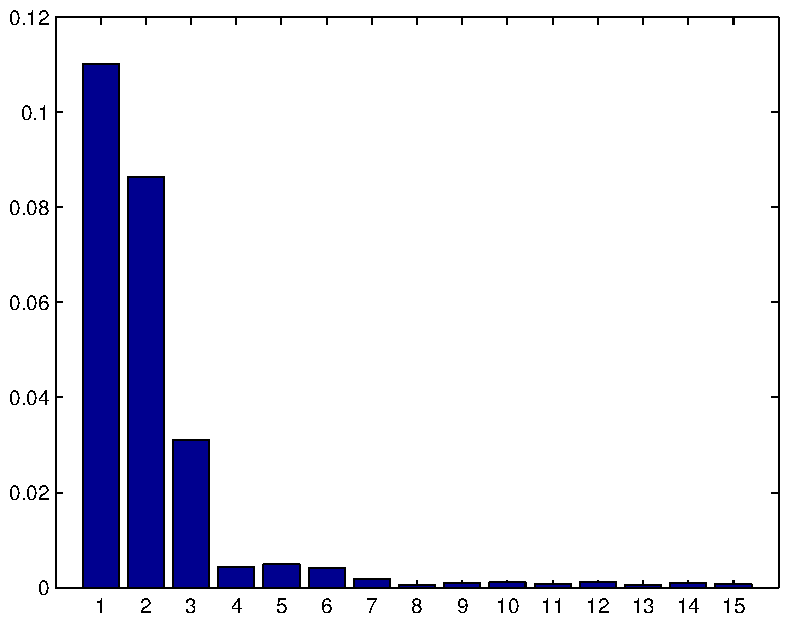
\includegraphics[width=0.145\textwidth]{../diagrams/Yale1Face/scales}
	\label{fig:yaleOneFaceScales}
}
\hspace{-5pt}
\subfigure[]{
	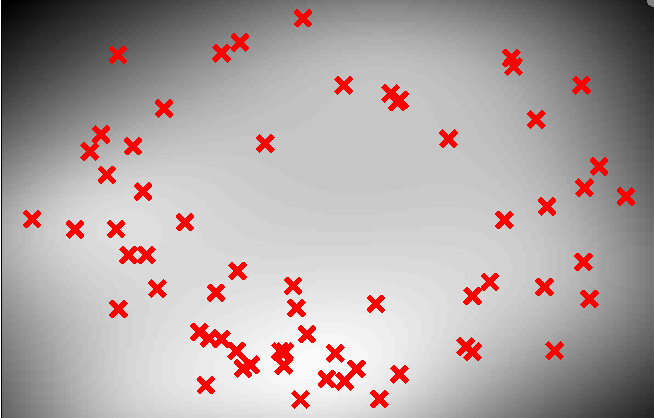
\includegraphics[width=0.145\textwidth]{../diagrams/Yale1Face/X21}
	\label{fig:yaleOneFaceX21}
}
\hspace{-5pt}
\subfigure[]{
	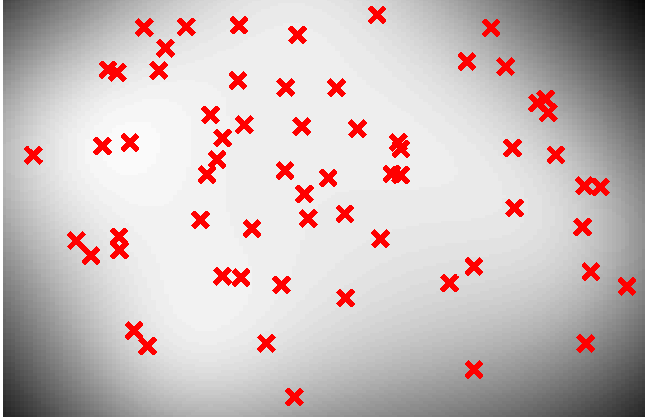
\includegraphics[width=0.145\textwidth]{../diagrams/Yale1Face/X23}
	\label{fig:yaleOneFaceX23}
}
\end{center}
\vspace{-7pt}
\caption{\small{ \it
The weight set $\bfw$ associated with the learned latent space is shown in \subref{fig:yaleOneFaceScales}.
In figures \subref{fig:yaleOneFaceX21} and \subref{fig:yaleOneFaceX23} we plotted pairs of the $3$ most dominant
latent dimensions against each other (dimension 1 against 2 and 1 against 3 respectively).
}
}
\label{fig:yaleOneFace1}
\vspace{-8pt}
\end{figure}
\hspace{-6pt}

This suggests that latent feature indices $1,2$ and $3$ encode the information about the illumination condition.
Figure \ref{fig:yaleOneFaceScales} also shows that the latent dimensions with indices $4,5$ and $6$ have a very small but not negligible weight.
%These are retained by the model because
%apart from the illumination condition, there exist other minor differences among pictures of a single face, as the depicted %persons
These represent other minor differences between an individual's face pictures, as the subjects
often blink, slightly move or smile etc. 



\subsubsection{Shared latent spaces for multiple faces}

In this section we use our model, from now on referred to as \emph{Manifold Relevance Determination model (MRD)} for latent subspace learning. 
We selected the pictures corresponding to all illumination conditions of $3$ subjects and created a dataset $Y$, and similarly
for $Z$ (for $3$ different subjects).
In this way, we formed two datasets, $Y$ and $Z$, each consisting of all $64 \times 3$ images corresponding to
a set of three different faces, therefore, $Y, Z \in \mathbb{R}^{N \times D}$, $N = 192$, $D = 32,256$.
 We then aligned the datasets, so that each image from the
first dataset was randomly set to correspond to one of the three faces of the second dataset which are depicted in the same illumination condition. In that way, the model is not
explicitly forced to learn the correspondence between face characteristics.

\par The MRD model was initialised by concatenating the two datasets and then performing PPCA in $Q=14$ dimensions. After training, 
the dimensions of the learned latent space are weighted by the parameters of the generative mappings $f_Y$ and $f_Z$ as shown in figure \ref{fig:yale6SetsScales}.

\begin{figure}[ht]
\begin{center}
\subfigure[]{
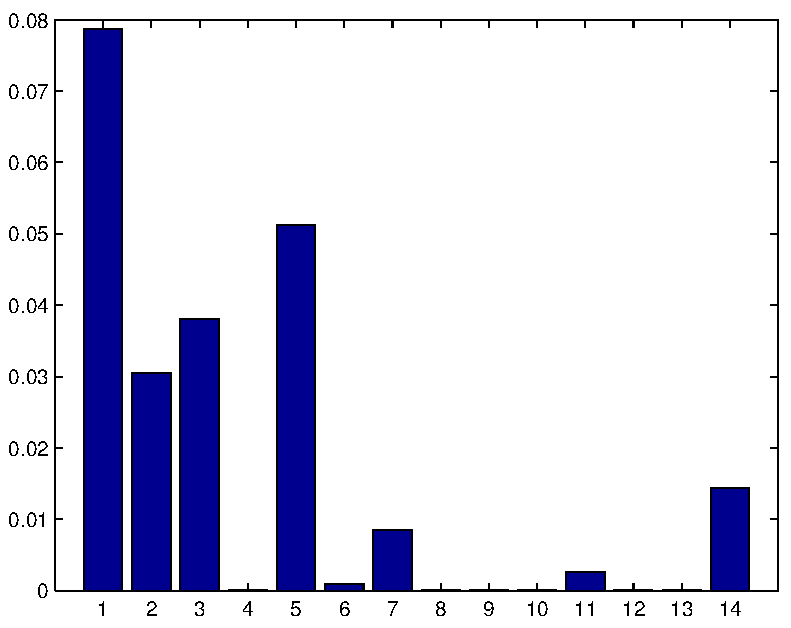
\includegraphics[width=0.18\textwidth]{../diagrams/Yale6Sets/scalesMod1}
	\label{fig:yale6SetsScales1}
}
\subfigure[]{
	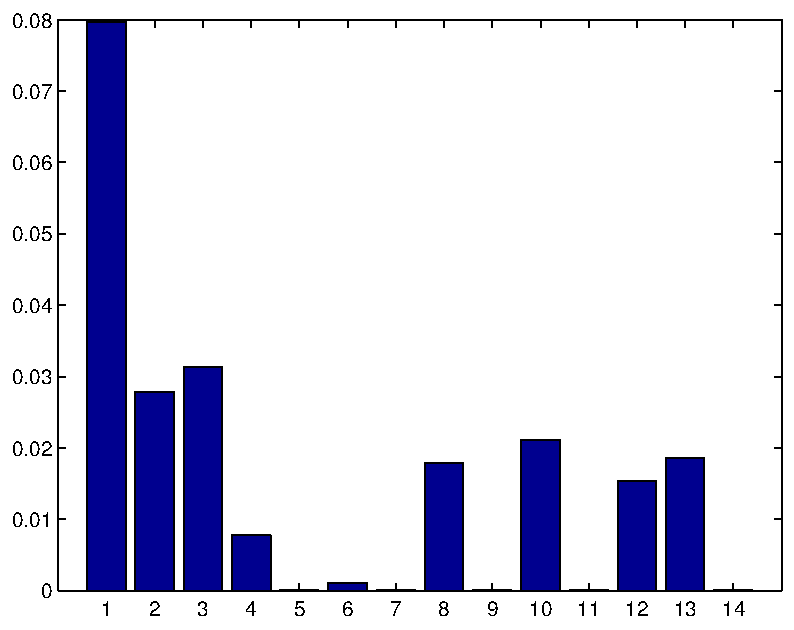
\includegraphics[width=0.18\textwidth]{../diagrams/Yale6Sets/scalesMod2}
	\label{fig:yale6SetsScales2}
}
\end{center}
\vspace{-9pt}
\caption{\small{ \it
The dimensions' weights, assigned for the first and second dataset 
in \subref{fig:yale6SetsScales1} and \subref{fig:yale6SetsScales2},
define a partitioning and ``soft'' sharing of the latent space. 
}}
\label{fig:yale6SetsScales}
\vspace{-8pt}
\end{figure}

The latent space is clearly segmented into a shared part, consisting of dimensions indexed as $1$,$2$ and $3$ 
\footnote{dimension 6 is also in the shared set but both models assigned a very small weight for that, as it encodes an almost negligible amount of information.}
and two private parts, consisting of dimensions indexed as $\{5,7,11,14 \}$ and $\{4,8,10,12,13 \}$ respectively. 
The $9$th feature of every latent point was found to be unnecessary for the generation of both output spaces.
What is more, 
the two models assigned almost (relatively) equal weights to the shared feature indices, and 
the shape of the shared latent space is similar to
the one found by the Bayesian GP-LVM (figure \ref{fig:yaleOneFace1}), as can be seen in figures \ref{fig:yale6SetsLatentSpace}\subref{fig:yale6SetsX12} and
\ref{fig:yale6SetsLatentSpace}\subref{fig:yale6SetsX13}.

This indicates that the shared space successfully encodes the information about
the position of the light source and not the face characteristics.
%as the random alignment that we performed forbade the algorithm from modelling commonalities between faces of the
%two different datasets.
 As for the private parts, these mainly correspond to disambiguating between faces of the same dataset. Indeed, plotting the largest two dimensions of
the first latent private subspace against each other reveals three clusters, corresponding to the three different faces within the dataset. 
Similarly to the standard Bayesian GP-LVM applied to a single face, here the private dimensions with the smaller weight
are the ones that model the minor differences introduced by the fact that the subject characteristics are slightly changed in several photos (due to blinking etc).

\hspace{-6pt}
\begin{figure}[ht]
\begin{center}
\subfigure[]{
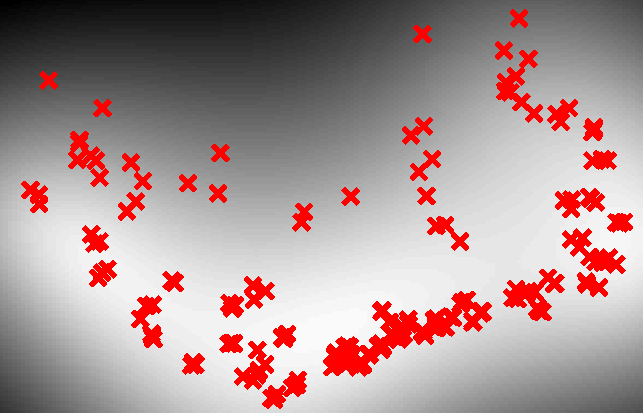
\includegraphics[width=0.145\textwidth]{../diagrams/Yale6Sets/mod1X_1_2}
	\label{fig:yale6SetsX12}
}
\hspace{-5pt}
\subfigure[]{
	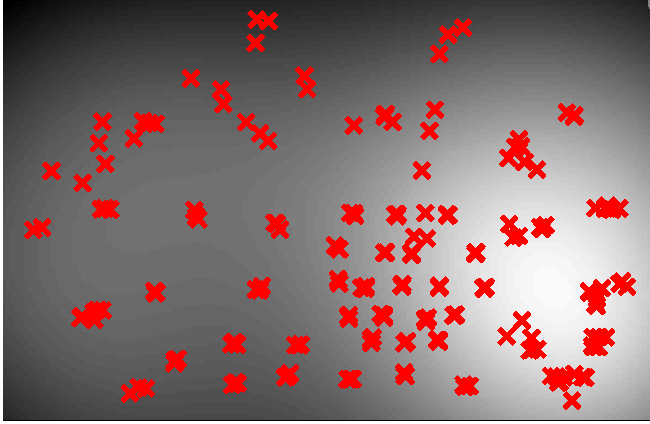
\includegraphics[width=0.145\textwidth]{../diagrams/Yale6Sets/mod1X_1_3}
	\label{fig:yale6SetsX13}
}
\hspace{-5pt}
\subfigure[]{
	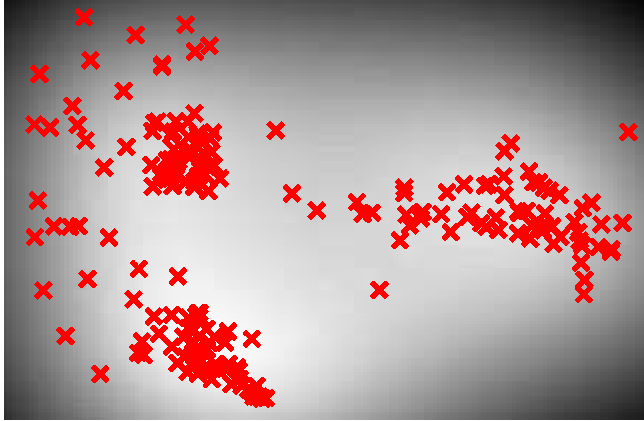
\includegraphics[width=0.145\textwidth]{../diagrams/Yale6Sets/mod1_X5_14}
	\label{fig:yale6SetsX5_14}
}
\end{center}
\vspace{-9pt}
\caption{\small{ \it
Projection of the shared latent space into dimensions $\{1,2\}$ and $\{1,3\}$ (figures
\subref{fig:yale6SetsX12} and \subref{fig:yale6SetsX13}) and projection of the $Y-$private dimensions $\{5,14\}$
(figure \subref{fig:yale6SetsX5_14}).
%which disambiguate between different faces in the first dataset.
 It is clear how the latent points in figure
\subref{fig:yale6SetsX5_14} form three clusters, each responsible for modelling one of the three faces in $Y$.
}}
\label{fig:yale6SetsLatentSpace}
\vspace{-8pt}
\end{figure}
\hspace{-6pt}


\par Given the above, it is obvious that the Manifold Relevance Determination model not only finds a very efficient and intuitive segmentation of the latent space, but it also
finds an effective dimensionality for each latent subspace. The Bayesian training allows for these procedures to be automated.

We can now confirm visually all of the subspaces' properties mentioned above and interpret their structure.
This is done by sampling a set of novel inputs $X_{samp}$ from each subspace and then mapping back to the observed data space using the
likelihood $p(Y|X_{samp})$, thus obtaining novel outputs (images).
%Being able to do so is an important advantage of our method (which is generative), because it also means that we can generate novel datapoints from the trained model.
%The intuitive segmentation of the latent space also helps towards this direction. 
To better understand what kind of information is encoded in each of the dimensions
of the shared or private spaces, we sampled new latent points by varying only one dimension at a time, while keeping the rest fixed. 

The first two rows of figure \ref{fig:yale6SetsInterpolation} show some of the outputs obtained after sampling across each of the shared dimensions $1$ and $3$ respectively, which clearly encode the coordinates of the light source,
whereas dimension $2$ was found to model the overall brightness. The sampling procedure can intuitively be thought as a walk in the space shown in figure \ref{fig:yale6SetsLatentSpace}\subref{fig:yale6SetsX13} from left to right and from the bottom to the top. Although the set of learned latent inputs is discrete, the corresponding latent subspace is continuous,
and we can interpolate images in new illumination conditions by sampling from areas where there are no training inputs (\ie in between the red crosses shown in figure \ref{fig:yale6SetsLatentSpace}).

% Using a generative model also allows us to sample new datapoints from the trained model. This is done by selecting a training input $\bfx_n$ (\ie one of
% the latent points corresponding to an existing, observed $\bfy_n$), and sampling one or more of its dimensions from the whole of the corresponding feature space,
% obtaining, thus, a novel input $\bfx_*$. We can then obtain novel outputs by using the likelihood $p(\bfy_n | \bfx_n)$. Figures \ref{}, \ref{} and \ref{} show some of the outputs obtained after
% sampling across each of the principle dimensions by hand. When the sampled $\bfx_*$ were close or exactly similar to training inputs, the corresponding output
% looks like one of the training datapoints, otherwise the output is novel. From the aforementioned figures, one can see that the two of the principal dimensions
% represent the change of the light source location along the $X$ and $Y$ axis respectively, whereas the third one is responsible for modelling the brightness.

Similarly, we can sample from the private subspaces and obtain novel outputs which interpolate the non-shared characteristics of the involved data. 
This results in a morphing effect across different faces, which is shown in the last row of figure \ref{fig:yale6SetsInterpolation}.
More examples and videos can be found in the supplementary material.


\begin{figure*}[ht]
\begin{center}
\subfigure{ 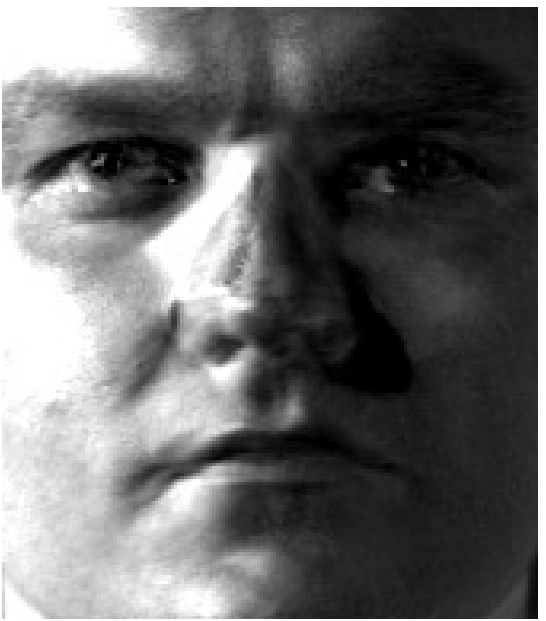
\includegraphics[width=0.09\textwidth]{../diagrams/Yale6Sets/lightInterpolation/X13_1000} }
\subfigure{ 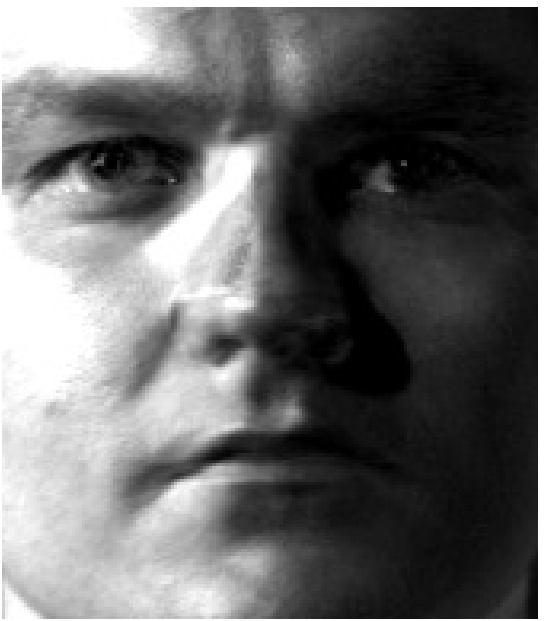
\includegraphics[width=0.09\textwidth]{../diagrams/Yale6Sets/lightInterpolation/X13_1009} }
\subfigure{ 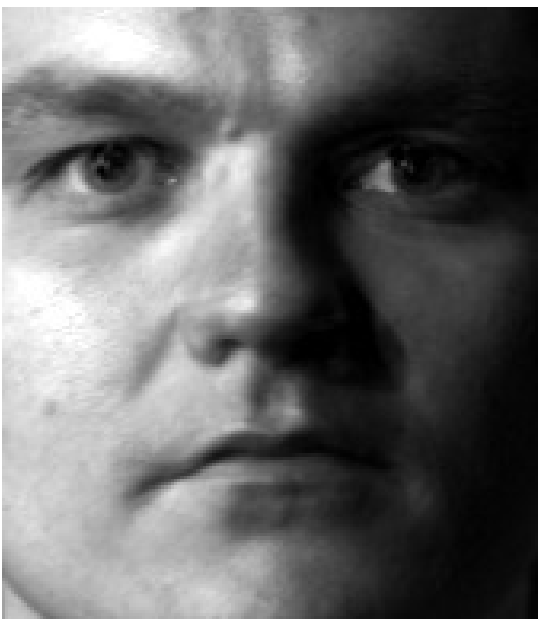
\includegraphics[width=0.09\textwidth]{../diagrams/Yale6Sets/lightInterpolation/X13_1021} }
\subfigure{ 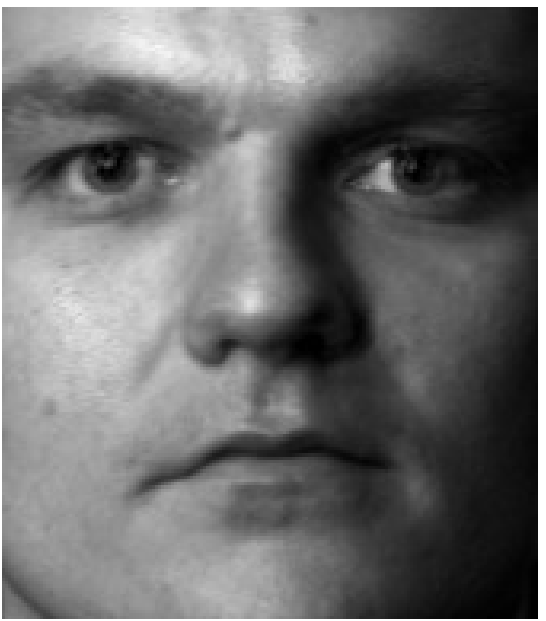
\includegraphics[width=0.09\textwidth]{../diagrams/Yale6Sets/lightInterpolation/X13_1022} }
\subfigure{ 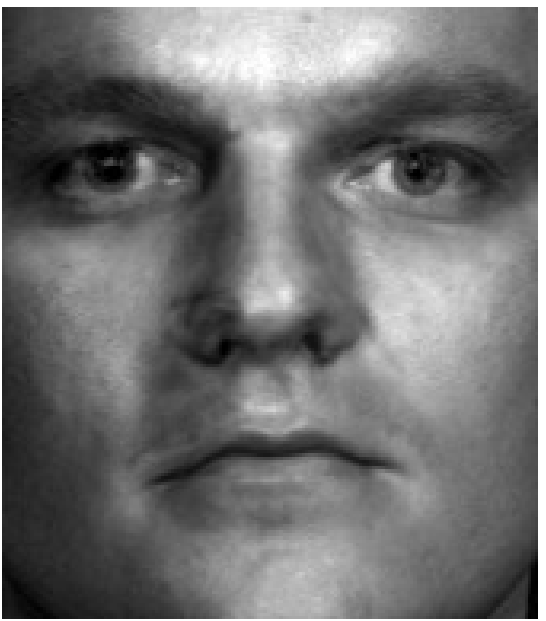
\includegraphics[width=0.09\textwidth]{../diagrams/Yale6Sets/lightInterpolation/X13_1036} }
\subfigure{ 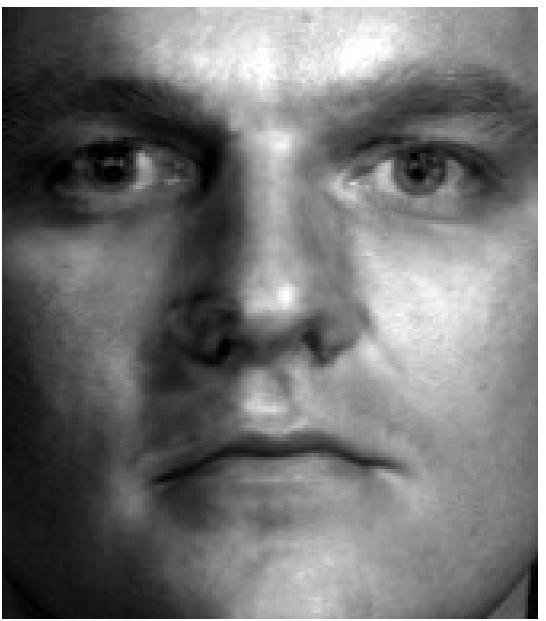
\includegraphics[width=0.09\textwidth]{../diagrams/Yale6Sets/lightInterpolation/X13_1040} }
\subfigure{ 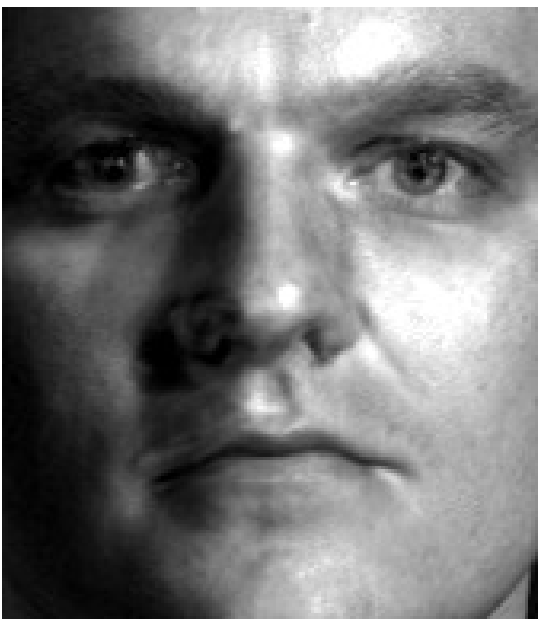
\includegraphics[width=0.09\textwidth]{../diagrams/Yale6Sets/lightInterpolation/X13_1046} }
\subfigure{ 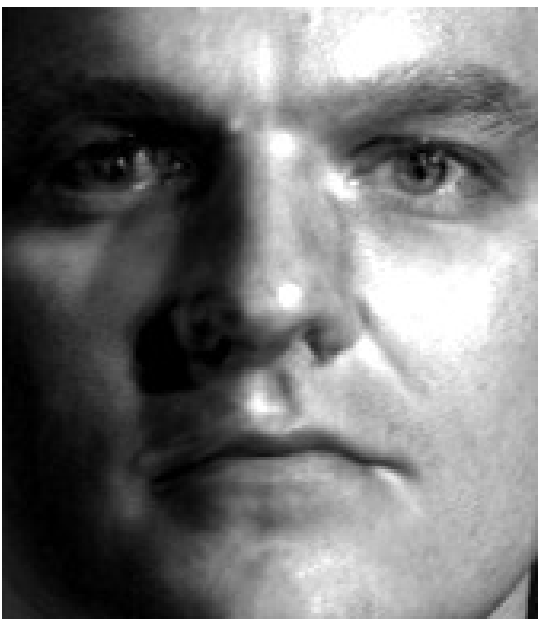
\includegraphics[width=0.09\textwidth]{../diagrams/Yale6Sets/lightInterpolation/X13_1055} }
\subfigure{ 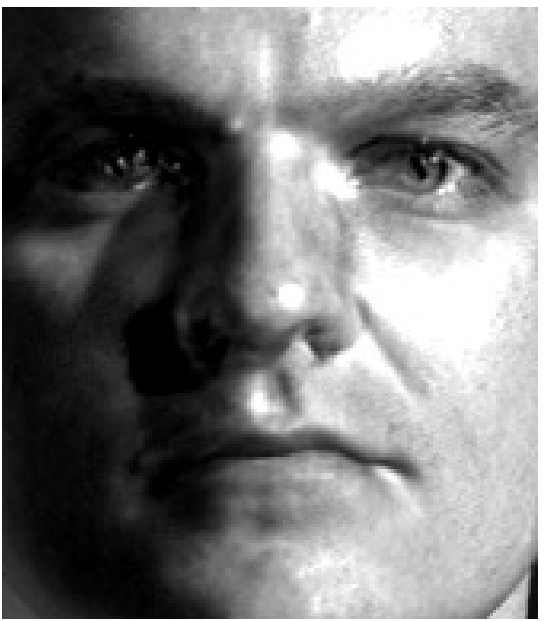
\includegraphics[width=0.09\textwidth]{../diagrams/Yale6Sets/lightInterpolation/X13_1063} }
\vspace{-8pt}
\newline
\subfigure{ 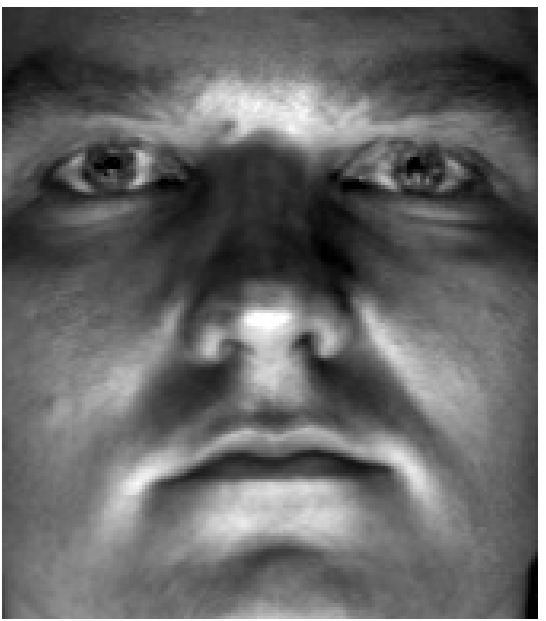
\includegraphics[width=0.09\textwidth]{../diagrams/Yale6Sets/lightInterpolation/X13_1064} }
\subfigure{ 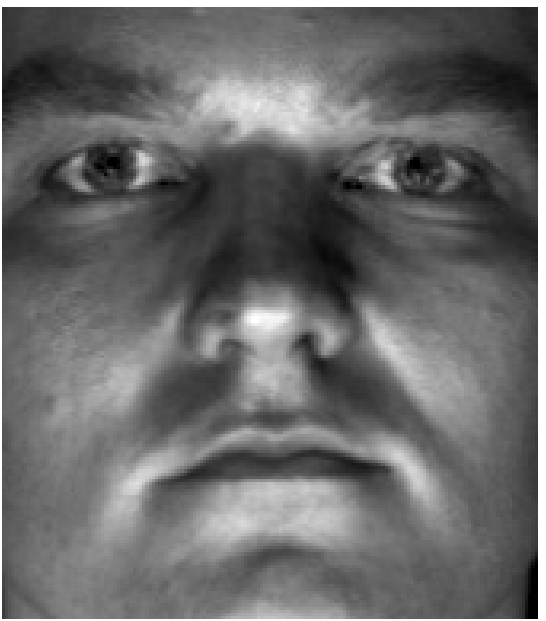
\includegraphics[width=0.09\textwidth]{../diagrams/Yale6Sets/lightInterpolation/X13_1072} }
\subfigure{ 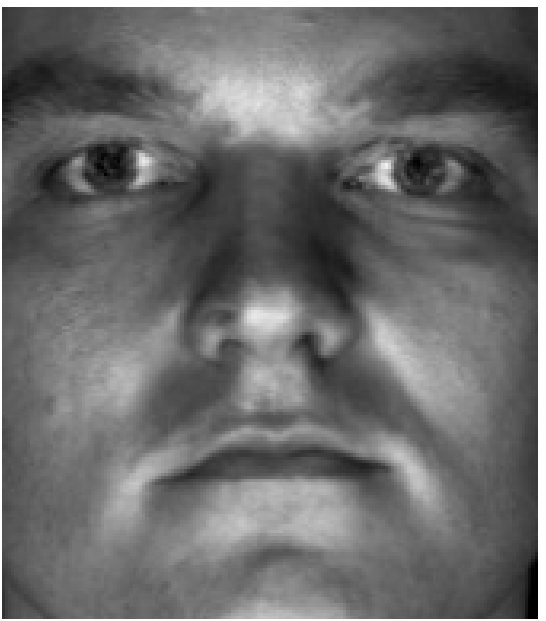
\includegraphics[width=0.09\textwidth]{../diagrams/Yale6Sets/lightInterpolation/X13_1079} }
\subfigure{ 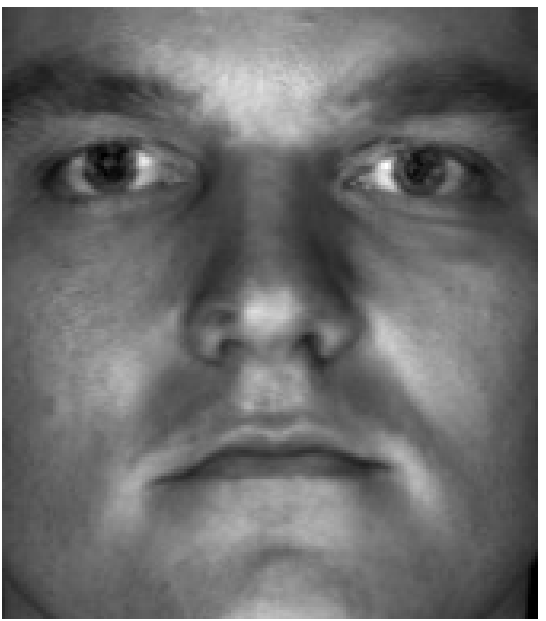
\includegraphics[width=0.09\textwidth]{../diagrams/Yale6Sets/lightInterpolation/X13_1085} }
\subfigure{ 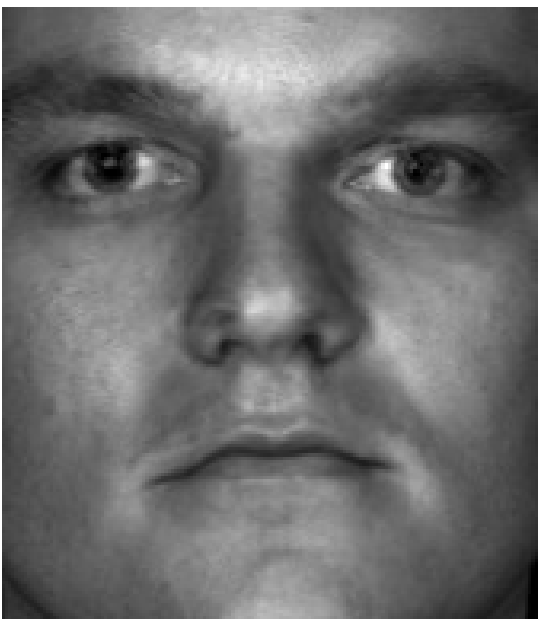
\includegraphics[width=0.09\textwidth]{../diagrams/Yale6Sets/lightInterpolation/X13_1095} }
\subfigure{ 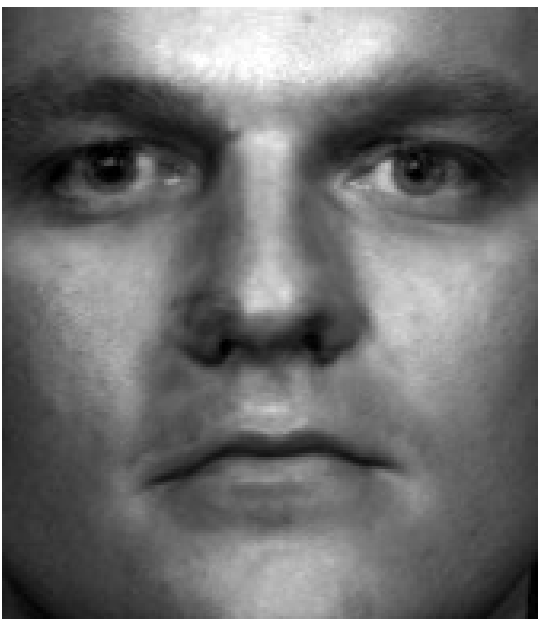
\includegraphics[width=0.09\textwidth]{../diagrams/Yale6Sets/lightInterpolation/X13_1110} }
\subfigure{ 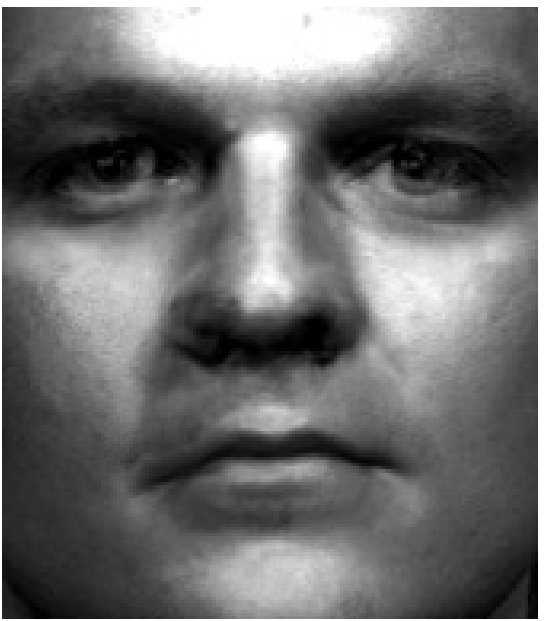
\includegraphics[width=0.09\textwidth]{../diagrams/Yale6Sets/lightInterpolation/X13_1125} }
\subfigure{ 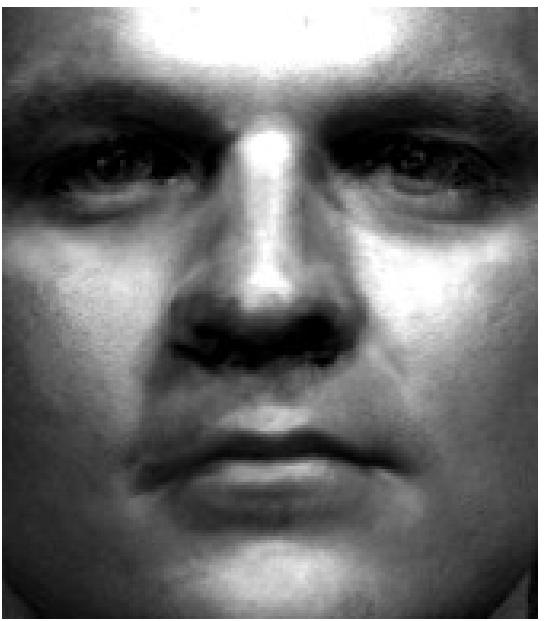
\includegraphics[width=0.09\textwidth]{../diagrams/Yale6Sets/lightInterpolation/X13_1137} }
\subfigure{ 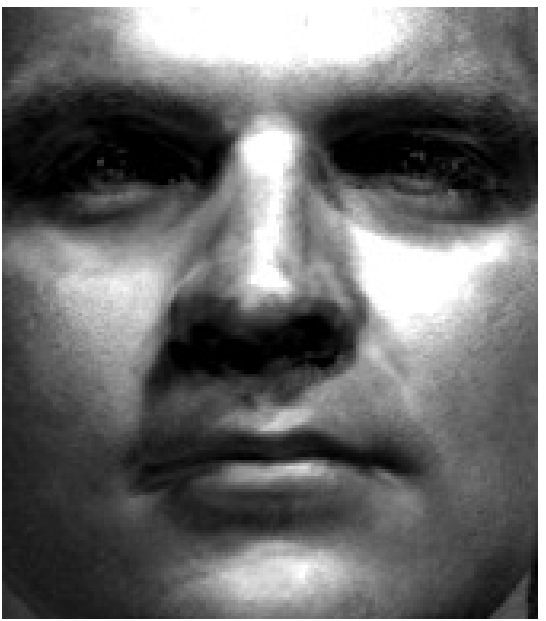
\includegraphics[width=0.09\textwidth]{../diagrams/Yale6Sets/lightInterpolation/X13_1149} }
\vspace{-8pt}
\newline
\subfigure{ 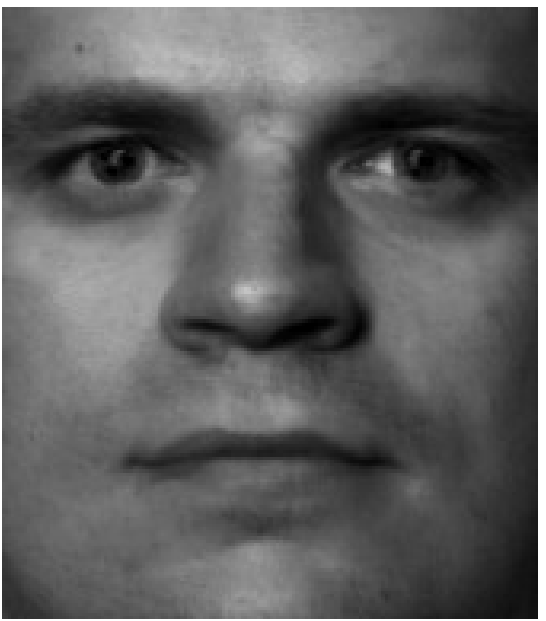
\includegraphics[width=0.11\textwidth]{../diagrams/Yale6Sets/morphing/1054} }
\subfigure{ 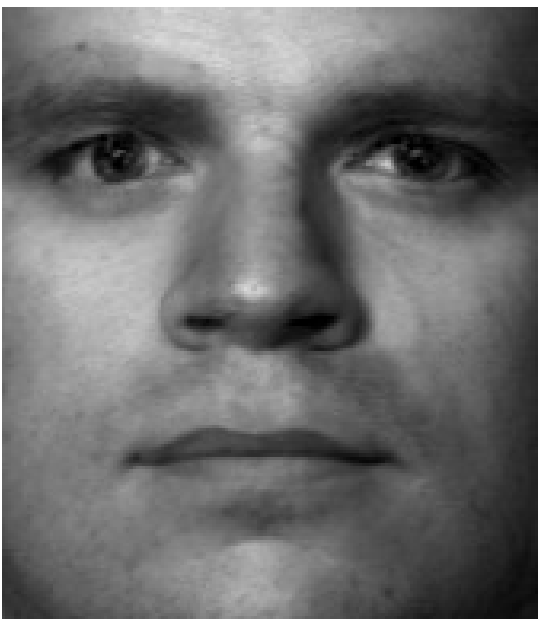
\includegraphics[width=0.11\textwidth]{../diagrams/Yale6Sets/morphing/1079} }
\subfigure{ 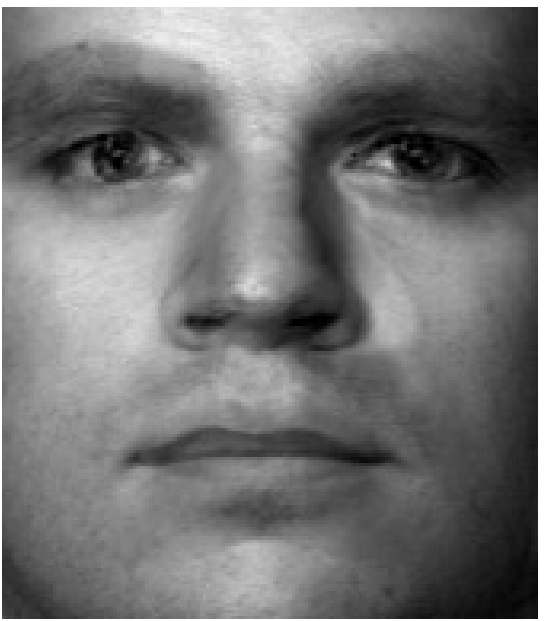
\includegraphics[width=0.11\textwidth]{../diagrams/Yale6Sets/morphing/1089} }
\subfigure{ 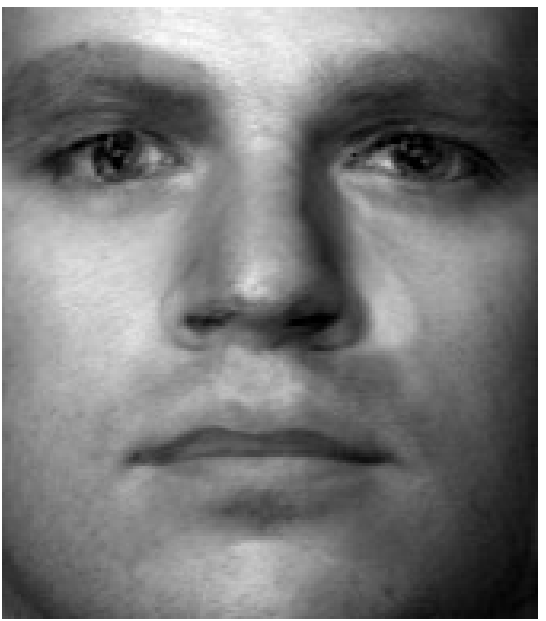
\includegraphics[width=0.11\textwidth]{../diagrams/Yale6Sets/morphing/1094} }
\subfigure{ 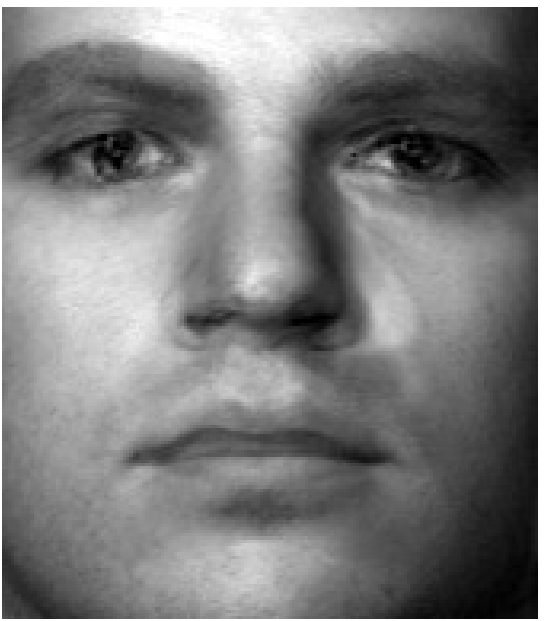
\includegraphics[width=0.11\textwidth]{../diagrams/Yale6Sets/morphing/1102} }
\subfigure{ 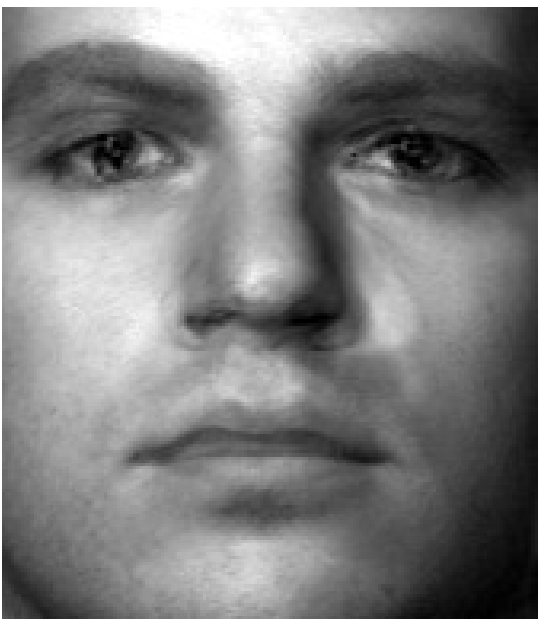
\includegraphics[width=0.11\textwidth]{../diagrams/Yale6Sets/morphing/1106} }
\subfigure{ 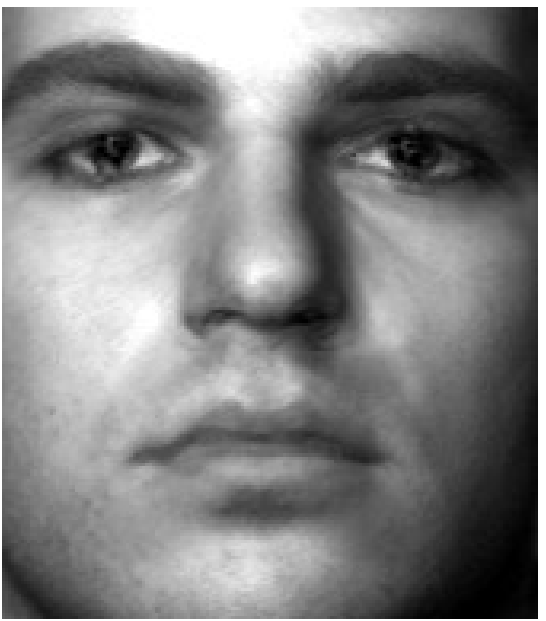
\includegraphics[width=0.11\textwidth]{../diagrams/Yale6Sets/morphing/1123} }
\end{center}
\vspace{-4pt}
\caption{\small{ \it
Sampling inputs to produce novel outputs.
First row shows interpolation between positions of the light source in the $x$ coordinate
and second row in the $y$ coordinate (elevation). Last row shows interpolation between
face characteristics to produce a morphing effect.
}}
\label{fig:yale6SetsInterpolation}
\vspace{-8pt}
\end{figure*}




\par As a final test, we confirm the efficient segmentation of the latent space into private and shared parts by automatically recovering all the illumination similarities found in
the training set.
 More specifically, given a datapoint $\bfy_n$ from the first dataset, we search the whole space of training inputs $X$ to find the $6$ Nearest Neigbours to the latent representation 
$\bfx_n$ of $\bfy_n$, based only on the shared dimensions. 
%In other words, we compare $x_{n,i}$ to all the rest $\{x_{n,j}\}_{n=1}^N$, where $i \neq j$ and $i,j$ belong to the set
% of the shared dimensions. 
 From these latent points, we can then obtain points in the output space of the second dataset, by using the likelihood $p(Z | X)$.
 As can be seen in figure \ref{fig:yale6SetsGrouping}, the model returns images which match
the illumination condition of the given image. Moreover, the fact that, typically, the first
neighbours of each given point correspond to outputs belonging to different faces, also indicates that
the shared latent space is ``pure'', and it does not encode similarities of face characteristics.
%\hspace{-6pt}
\begin{figure}[ht]
\begin{center}
\subfigure{ 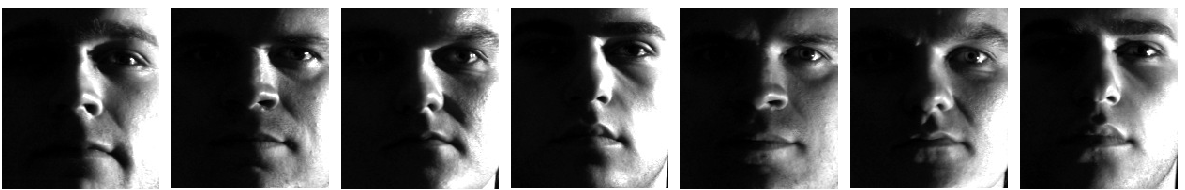
\includegraphics[width=0.47\textwidth]{../diagrams/Yale6Sets/grouping/givenMod2/122} }
 \vspace{-16pt}
 \newline
\subfigure{ 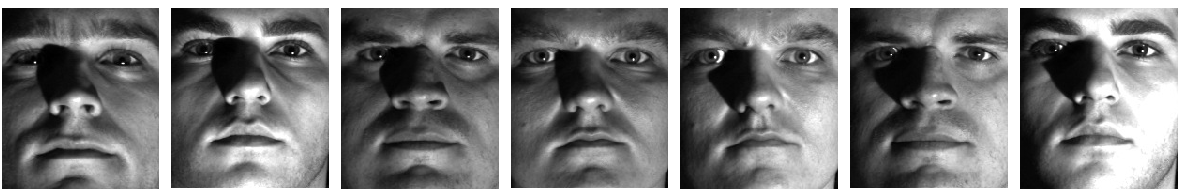
\includegraphics[width=0.47\textwidth]{../diagrams/Yale6Sets/grouping/givenMod2/107} }
 \vspace{-16pt}
 \newline
\subfigure{ 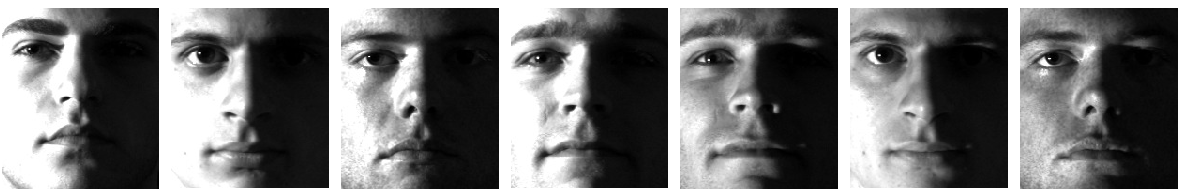
\includegraphics[width=0.47\textwidth]{../diagrams/Yale6Sets/grouping/givenMod1/24} }
 \vspace{-16pt}
 \newline
\subfigure{ 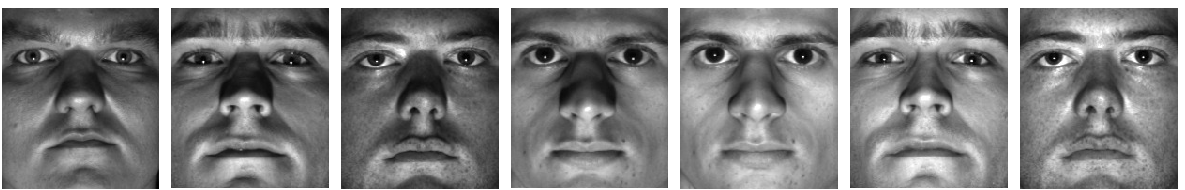
\includegraphics[width=0.47\textwidth]{../diagrams/Yale6Sets/grouping/givenMod1/70} }
 \vspace{-16pt}
 \newline
\end{center}
\vspace{-9pt}
\caption{\small{ \it
Given the images of the first column, the model searches only in the shared latent space to find the pictures of the opposite dataset
which have the same illumination condition. The images found, are sorted in columns
$2$ - $7$ by relevance.
}}
\label{fig:yale6SetsGrouping}
\vspace{-8pt}
\end{figure}

%\hspace{-6pt}

%%%% THE FIRST NN is the same latentn point, we should look from NN2 and so on.


\subsection{Human motion data}

For our second experiment, we consider 
a set of $3$D human poses and associated silhouettes,
coming from the dataset of Agarwal and Triggs \cite{Agarwal:pose06}. We used a subset of
$5$ sequences, totalling $649$ frames, corresponding to walking motions in various directions and patterns.
A separate walking sequence of $158$ frames was used as a test set.
Each pose is represented by a $63-$dimensional vector
of joint locations and each
silhouette is represented by a $100-$dimensional vector of HoG features.

\par Given the test silhouette features, we used our model to generate the corresponding
poses. This is a challenging task, since the data are multi-modal, \ie a silhouette representation
may be generated from more than one poses (\eg figure \ref{fig:humanPoseAmbiguity}). 

\begin{figure}[ht]
\begin{center}
%  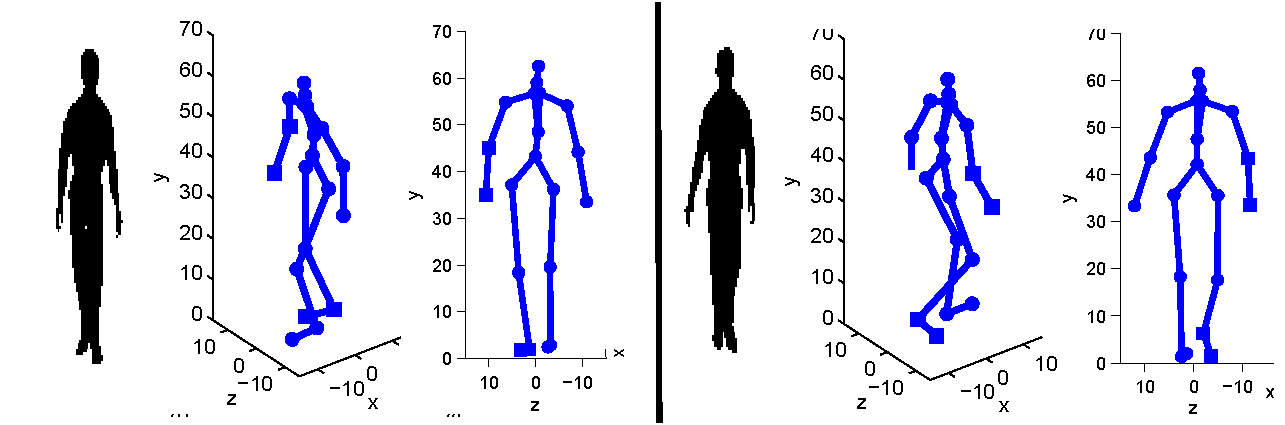
\includegraphics[width=0.43\textwidth]{../diagrams/humanPose/ambiguity2FinalCombined3}
  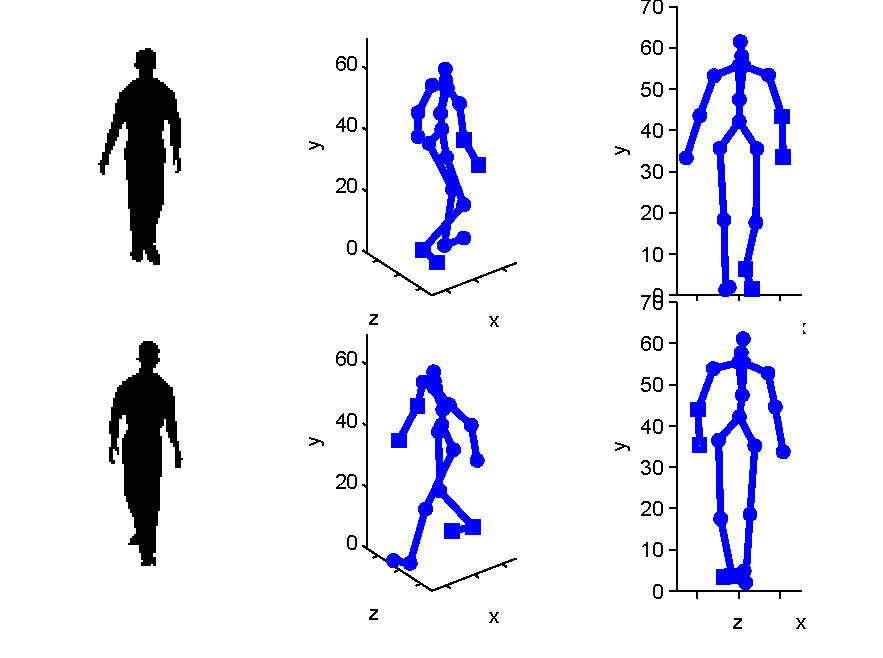
\includegraphics[width=0.35\textwidth]{../diagrams/humanPose/newAmbiguity}
\end{center}
\vspace{-9pt}
\caption{\small{ \it
Although the two poses in the second column are very dissimilar, they correspond to resembling silhouettes
that have similar feature vectors. This happens because the $3$D information is lost in the silhouette space,
as can also be seen in the third column, depicting the same poses from the silhouettes' viewpoint.}}
\label{fig:humanPoseAmbiguity}
\vspace{-4pt}
\end{figure}

As described in section \ref{inference}, given $\bfy^*$, one of the $N_*$ test silhouettes, our model optimises a test latent point $\bfx^*$ and finds
 a series of $K$ candidate initial training inputs $ \{ \bfx_{NN}^{(k)} \}_{k=1}^K$, sorted according to their similarity to $\bfx^*$, taking into account only the shared dimensions. 
 Based on these initial latent points, it then generates a sorted series of $K$ poses $\{ \bfzi^{(k)} \}_{k=1}^K$. For the dynamical version of our model,
all the test points are considered together and the predicted $N_*$ outputs are forced to form a smooth sequence.
 Our experiments showed that the initial training inputs $\bfx_{NN}$ typically correspond to silhouettes similar to the given one, something which
 confirms that the segmentation of the latent space is efficient. However, when ambiguities arise, as the example
 shown in figure \ref{fig:humanPoseAmbiguity}, the non-dynamical version of our model has no way of selecting the right one, since all points
 of the test sequence are treated independently. But when the dynamical version is employed, the model forces the whole set of training and test inputs to create smooth paths in the latent space, as can be seen in figure \ref{fig:humanPoseLatentSpaces}. In other words,
 the dynamics disambiguate the model.  

\begin{figure}[ht]
\begin{center}
\subfigure[]{ 
\includegraphics[width=0.18\textwidth]{../diagrams/humanPose/latentSpaceStatic} 
\label{fig:latentSpaceStatic}
} \hspace{-3pt}
\subfigure[]{ 
\includegraphics[width=0.18\textwidth]{../diagrams/humanPose/latentSpaceDynCropped} 
\label{fig:latentSpaceDyn}
}
\end{center}
\vspace{-9pt}
\caption{\small{ \it Projection of the latent space discovered for the non-dynamical model \subref{fig:latentSpaceStatic}
and for the dynamical model \subref{fig:latentSpaceDyn} onto their two principal dimensions.
}
}
\label{fig:humanPoseLatentSpaces}
\vspace{-3pt}
\end{figure}


Indeed, as can be seen in figure \ref{fig:humanPoseAmbiguityTest}, our method is forced to select a candidate training input $\bfx_{NN}$ for initialisation which does not necessarily
correspond to the training silhouette that is most similar to the test one. 
%
%In other words, the predicted pose is generated by a latent point which is not
%necessarily initialised in the latent point that is found by Nearest Neighbour in the silhouette space. 
%
What is more, if we assume that the test \emph{pose} $\bfzi^*$ is known and seek for its nearest training neighbour in the pose space, we find that the corresponding silhouette
is very similar to the one found by our model, which is only given information in the silhouette space.

\begin{figure}[ht]
\begin{center}
  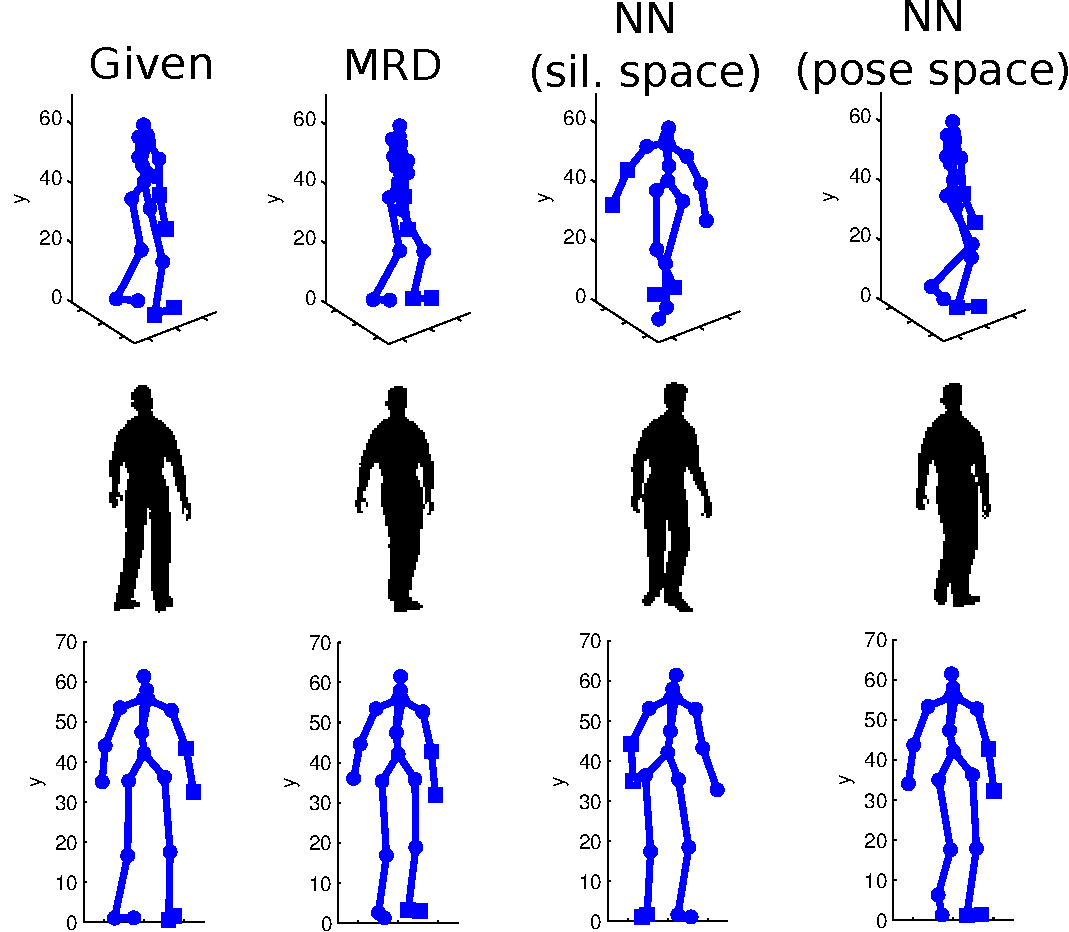
\includegraphics[width=0.35\textwidth]{../diagrams/humanPose/ambiguityTest}
\end{center}
\caption{\small{\it Given the HoG features for the test silhouette in column one, we predict the corresponding pose using the dynamical version of MRD and Nearest Neighbour in the silhouette space
obtaining the results in the first row, columns 2 and 3 respectively. The last row is the same as the first one, but the poses are rotated
to highlight the ambiguities. Notice that the silhouette shown in the second row for MRD does not correspond exactly to the pose
of the first row, as the model generates only the pose given a test silhouette. Instead, it is the training silhouette which MRD chose to initialise with, by performing
Nearest Neighbour in the shared latent space. 
We also found the Nearest Neighbour of the training \emph{pose} (column 4) given the test pose, so as to show that the corresponding silhouette is very similar to the one
selected by MRD for initialisation.
}}
\label{fig:humanPoseAmbiguityTest}
\end{figure}

\par Given the above, we quantify the results and compare our method
with linear and Gaussian process regression and Nearest Neighbour in the silhouette space. We also compared against
the Shared GP-LVM \cite{Ek:2008up, Ek:2009vv} which optimises the latent points using MAP and, therefore, requires an initial factorisation
of the inputs to be given a priori. 
The errors shown in table \ref{humanMotionTable} as well as the video provided as supplementary  material show that MRD
performs better than the other methods in this task.



\begin{table}[h]
\label{humanMotionTable}
\begin{center}
\begin{tabular}{|l|l|}
\hline
						 	   & Error \\ \hline \hline
Mean Training Pose		       & 6.16   \\ \hline
Linear Regression		       & 5.86   \\ \hline
GP Regression 			       & 4.27   \\ \hline
Nearest Neighbour (sil. space) & 4.88  \\ \hline
\textcolor{Gray}{Nearest Neighbour (pose space)} & \textcolor{Gray}{2.08}   \\ \hline
Shared GP-LVM				       & 5.13    \\ \hline
MRD	without Dynamics       & 4.67   \\ \hline
MRD with Dynamics	       & \textbf{2.94}    \\ \hline
\end{tabular}
\end{center}
\caption{
\small{ \it
The mean of the Euclidean distances of the joint locations between the predicted and the true poses.
The Nearest Neighbour in the pose space
is not a fair comparison, but is reported here as it provides some insight about the
lower bound on the error that can be achieved for this task.
}}
\end{table}










\section{Conclusions \label{conclusions}}
%% Many applications in computer vision and related fields are concerned
%% with modelling in scenarios where multiple streams of information of
%% the same underlying phenomenon are available. Further, the data is
%% often very high dimensional with enormous redundancies.
%Such a representation often means that the data
%is distributed on or close to a manifold through the observed
%parametrization.  
We have presented a new factorized latent variable model for multi
view data.  The model automatically factorizes the data using
variables representing variance that exists in each view separately
from variance being specific to a particular view. 
%% that automatically factorizes the latent space into variables that
%% are either shared or specific to one of the views of the
%% data.
% We introduced a relaxation to the discrete segmentation
%% of the latent representation 
% and allow for a ``softly'' shared latent space.
%The model learns the structure of the latent space variationally,
% allowing it to incorporate prior distributions for the latent space. 
The model learns a distribution over the latent points
variationally. This allows us to to automatically find the
dimensionality of the latent space as well as to incorporate prior
knowledge about its structure.
%
As an example, we showed how dynamical priors can be included on the latent
space. This allowed us to use temporal continuity to disambiguate the
model's predictions in an ambiguous human pose estimation problem.
%
%We exploited the factorization to perform human
%pose estimation in an ambiguous setting.
% where the model separates the variance in the pose
%space that can be determined from the image observations from the one
%that is ambiguous. 
% Our model allows for dynamical priors to be
% incorporated when learning it. This allowed us to disambiguate
% in the pose estimation example. 
%
The model is capable of learning from extremely high-dimensional
data. We illustrated this by learning a model directly on the pixel
representation of an image. Our model is capable of learning a compact
an intuitive representation of such data which we exemplified by
generating novel images by sampling from the latent representation in a
structured manner.
%% applying it to images of several different
%% faces under the same set of lighting conditions. Images of faces from
%% novel lighting directions or with novel appearance could be
%% synthesized by sampling from the corresponding latent space.
%
%The model is capable of learning from
%extremely high-dimensional data. By applying it to images of
%several different faces under the same set of lighting conditions the model
%correctly finds the generating low-dimensional parameters of the data
%separated into facial appearance and illumination direction. From the
%resulting model we showed how images of faces from novel lighting
%directions or with novel facial characteristics could be synthesized.
%
%
Finally, we showed how a generative model with discriminative
capabilities can be obtained by treating the observations and class labels
of a dataset as separate modalities.  

% As future work, we envisage
% approaches with more sophisticated ways of directly constraining the
% latent space through priors. 
% %In classification scenarios, for
% %example, we could consider a latent space prior evaluated at the class
% %labels.
%  Further, it would be interesting to explore the possibility of
% incorporating different latent space constraints for each different
% observed modality.


%%% Local Variables: 
%%% mode: latex
%%% TeX-master: "../svargplvmICML2012"
%%% End: 



\section*{Acknowledgments}
Research was partially supported by the University of Sheffield Moody endowment fund and the Greek State Scholarships Foundation (IKY).
We would like to thank the reviewers for their useful feedback.



\small
\bibliography{svargplvmICML2012,other,lawrence,zbooks}
\bibliographystyle{icml2012}
%}

%\newpage
 \begin{center}
 \begin{Large}
 \textbf{
% Gaussian Process Dynamical Systems\\
 Appendix
 } \\
 \end{Large}
% \noindent \newline
% \textbf{Andreas Damianou, Michalis Titsias, Neil Lawrence}
 \end{center}
\appendix
\section{Derivation of the variational bound}

We wish to approximate the marginal likelihood:
\begin{equation}
\label{marginalLikelihoodSuppl}
p(Y | \bft) =  \int p( Y , F, X| \bft) \intd  X \intd F,
\end{equation}
by computing a lower bound:
\begin{align}
\mathcal{F}_v(q, \boldsymbol \theta) = {}& \int q(\mathit{\Theta}) \log 
		\frac{ p(Y , F , \mathit{X} | \mathbf{t})}
			 {q(\mathit{\Theta})}  \intd  X \intd F.
% 	    \nonumber \\
% 	      = {}& \sum_{d=1}^D \int q(\Theta) \log \left( p(\bfy_d | \bff_d) p(\bff_d | X) \right) dX d \bff_d -
% 		    \int q(\Theta) \frac{p(X|\bft)}{q(\Theta)} dX
		 \label{jensens1Suppl}
\end{align}
%
This can be achieved by first augmenting the joint probability density of our model with inducing inputs $\tilde{X}$ along with their corresponding function values $U$:
\begin{equation}
 \label{augmentedJointSuppl}
p(Y,F, U,X,\tilde{X} | \bft) = \prod_{d=1}^D p(\mathbf{y}_d | \mathbf{f}_d) p(\mathbf{f}_d | \mathbf{u}_d, \mathit{X})
p(\bfu_d | \tilde{X})  p(X | \mathbf{t})
\end{equation}
where $p(\bfu_d | \tilde{X}) = \prod_{d=1}^D \mathcal{N} \left( \bfu_d | \mathbf{0}, K_{MM} \right)$ . For simplicity, $\tilde{X}$ is dropped from our
expressions for the rest of this supplementary material. Note that after including the inducing points, $p(\bff_d | \bfu_d, X)$
remains analytically tractable and it turns out to be \cite{rasmussen-williams}):
\begin{equation}
 \label{priorF2Suppl}
p(\bff_d | \bfu_d, X) =  \mathcal{N}  \left( \bff_d | K_{NM} K_{MM}^{-1} \bfu_d , K_{NN} - K_{NM} K_{MM}^{-1} K_{MN} \right).
\end{equation}
For tractability, we now define a variational density $q(\Theta)$:
\begin{equation}
\label{varDistrSuppl}
q(\mathit{\Theta}) = q(F, U,X) = q(F | U, X) q(U) q(X) = \prod_{d=1}^D p(\bff_d | \bfu_d, X )q(\bfu_d) q(X),
\end{equation}
%
%
where $q(X) = \prod_{q=1}^Q \mathcal{N} \left( \bfx_q | \bfmu_q, S_q \right)$. 
%
Now, we return to \eqref{jensens1Suppl} and replace the joint distribution with its augmented version \eqref{augmentedJointSuppl} and the variational distribution with its factorised version \eqref{varDistrSuppl}:
\begin{align}
\mathcal{F}_v(q, \boldsymbol \theta) = {}& \int q(\mathit{\Theta}) \log 
		\frac{ p(Y,F, U,X | \bft)}
			 {q(F, U,X)}  \intd  X \intd F,
 	    \nonumber \\
= {}& \int \prod_{d=1}^D p(\bff_d | \bfu_d, X )q(\bfu_d) q(X) 
	    \log  \frac{\prod_{d=1}^D p(\mathbf{y}_d | \mathbf{f}_d) \cancel{p(\mathbf{f}_d | \mathbf{u}_d, \mathit{X})}
						p(\bfu_d | \tilde{X})  p(X | \mathbf{t})}
 	      		   {\prod_{d=1}^D \cancel{p(\bff_d | \bfu_d, X )}q(\bfu_d) q(X)}   \intd  X \intd F \nonumber \\
= {}& \int \prod_{d=1}^D p(\bff_d | \bfu_d, X )q(\bfu_d) q(X) 
		\log  \frac{\prod_{d=1}^D p(\mathbf{y}_d | \mathbf{f}_d) p(\bfu_d | \tilde{X})}
				   {\prod_{d=1}^D q(\bfu_d) q(X)}   \intd  X \intd F \nonumber \\
- {}& \int \prod_{d=1}^D  q(X)   \log \frac{q(X)}{p(X | \mathbf{t})}   \intd  X \nonumber \\
= {}& \hat{\mathcal{F}}_v - \text{KL}(q \parallel p), \label{jensensSuppl}
\end{align}
%
with:
 \begin{equation}
\hat{\mathcal{F}}_v = 
\sum_{d=1}^D \left( 
    \int q(\bfu_d) q(X) \left\langle \log p(\bfy_d | \bff_d) \right\rangle_{p(\bff_d | \bfu_d, X)} d\bfu_d \; dX +
					   \log \left\langle \frac{p(\bfu_d)}{q(\bfu_d)} \right\rangle_{q(\bfu_d)} 
  \right) = \sum_{d=1}^D \hat{\mathcal{F}}_d
\end{equation} 

Both terms in \eqref{jensensSuppl} are analytically tractable, with the first having the same analytical solution as the one derived in \cite{BayesianGPLVM}. Further calculations in the the $\hat{\mathcal{F}}_v$ term reveal that the optimal setting for $q(\bfu_d)$ is also a Gaussian. More specifically, 
we have:
\begin{align}
\hat{\mathcal{F}}_v={}& \int q(\bfu_d) \log \frac{e^{\la \log N \left( \bfy_d | \bfa_d, \beta^{-1} I_d \right) \ra_{q(X)}}
		p(\bfu_d)}{q(\bfu_d)} d\bfu_d - A \label{boundFAnalytically5}
\end{align}
where $A$ is a collection of remaining terms and $\bfa_d$ is the mean of \eqref{priorF2Suppl}.
\eqref{boundFAnalytically5} is a KL-like quantity and, therefore, $q(\bfu_d)$ is optimally set to be the quantity appearing in the numerator of the above equation. So:
%:
% \begin{equation}
% q(\bff_{*,d}^m | X_*) = \mathcal{N}(\bff_{*,d}^m| \beta K_{N_* M} 
% (K_{MM} + \beta \Psi_2)^{-1} \Psi_1^{T} \bfy_d, K_{N_* N_*} - 
%  K_{N_* M} \left[ K_{M M}^{-1}  - (K_{M M} + \beta \Psi_2)^{-1} \right] 
%  K_{N_* M}^{T}),
% \end{equation}
% exactly as in \cite{BayesianGPLVM}.
\begin{equation}
\label{qu}
q(\bfu_d) = e^{\la \log \mathcal{N} \left( \bfy_d | \bfa_d, \beta^{-1} I_d \right) \ra_{q(X)}}
		p(\bfu_d) ,
\end{equation}
exactly as in \cite{BayesianGPLVM}. This is a Gaussian distribution since $p(\bfu_d ) = \mathcal{N} (\bfu_d | \mathbf{0}, K_{MM} )$.

\par
The complete form of the Jensen's lower bound turns out to be:
\begin{align}
\mathcal{F}_v(q, \boldsymbol \theta) = {}& \sum_{d=1}^{D} 
	\hat{\mathcal{F}}_d(q, \boldsymbol \theta) -  \text{KL}(q \parallel p) \nonumber \\
	= {}& 
	\sum_{d=1}^{D} 
		\log \left( 
		\frac{(\beta)^{\frac{N}{2}} \vert \mathit{K_{MM}} \vert ^\frac{1}{2} }
			 {(2\pi)^{\frac{N}{2}} \vert \beta \Psi_2 + \mathit{K_{MM}}  \vert ^\frac{1}{2} } 	
		 e^{-\frac{1}{2} \mathbf{y}^{T}_{d} W \mathbf{y}_d} 
		 \right) -
		 \frac{\beta \psi_0}{2} + \frac{\beta}{2} 
		 \text{Tr} \left( \mathit{K_{MM}^{-1}} \Psi_2 \right)  \nonumber \\
{}&	- \frac{Q}{2} \log \vert \mathit{K_t} \vert - \frac{1}{2} \sum_{q=1}^{Q}
	  \left[ \text{Tr} \left( \mathit{K_t}^{-1} \mathit{S_q} \right)	  
	  	   + \text{Tr} \left( \mathit{K_t}^{-1} \boldsymbol \mu_q \boldsymbol \mu_q^T \right) \right] 
	 + \frac{1}{2} \sum_{q=1}^Q \log \vert \mathit{S_q} \vert + const  \label{boundFinal}
\end{align}
where the last line corresponds to the KL term. Also:
\begin{equation}
\label{psis}
\Psi_0 = \text{Tr}(\langle \mathit{K_{NN}} \rangle_{q(\mathit{X})}) \;, \;\;
\Psi_1 = \langle \mathit{K_{NM}} \rangle_{q(\mathit{X})} \;, \;\;
\Psi_2 = \langle \mathit{K_{MN}} \mathit{K_{NM}} \rangle_{q(\mathit{X})}
\end{equation}
The $\Psi$ quantities can be computed analytically as in \cite{BayesianGPLVM}.


%-------------------------

\section{Derivatives of the variational bound}
Before giving the expressions for the derivatives of the variational bound \eqref{jensensSuppl},
it should be reminded that the variational parameters $\mu_q$ and $S_q$ (for all $q$s) have been
reparametrized as $S_q = \left( \mathit{K}_t^{-1} + diag(\boldsymbol \lambda_q) \right)^{-1}  \text{ and }   \boldsymbol \mu_q = K_t \bar{\boldsymbol \mu}_q$, where the function $diag(\cdot)$ transforms a vector into a square diagonal matrix and vice versa. Given the above, the set of the parameters to be optimised is 
$( \boldsymbol \theta_f, \boldsymbol \theta_x, \{ \bar{\bfmu}_q, \boldsymbol \lambda_q \}_{q=1}^Q, \tilde{X})$. The gradient w.r.t the inducing points $\tilde{X}$, however, has exactly the same form as for $\boldsymbol \theta_f$ and, therefore, is not presented here. Also notice that from now on we will often use the term ``variational parameters'' to refer to the new quantities $\bar{\bfmu}_q$ and $\boldsymbol \lambda_q$. 

\textbf{Some more notation:} 
\begin{enumerate}
\item $\lambda_q$ is a scalar, an element of the vector $\boldsymbol \lambda_q$ which, in turn, is the main diagonal of the diagonal matrix $\Lambda_q$. 
%\item$\lambda_m \triangleq \boldsymbol \lambda_{q;m}$, i.e. the $m$-th element of the vector $\boldsymbol \lambda_q$ (thus, an instantiation of $\lambda_q$)
\item $S_{ij} \triangleq S_{q;ij}$ the element of $S_q$ found in the $i$-th row and $j$-th column.
\item $\mathbf{s}_q \triangleq \lbrace S_{q;ii} \rbrace_{i=1}^N$, i.e. it is a vector with the diagonal of $S_q$.
%\item $s_i$ is the $i$-th element of $\mathbf{s}_q$.
%\item $diag(\mathbf{s}_q)$ is a matrix full of zeros apart from the main diagonal which contains the vector $\mathbf{s}_q$.
\end{enumerate}

\subsection{Derivatives w.r.t the variational parameters}
\begin{equation}
    \label{derivVarParamSuppl}
\frac{\vartheta \mathcal{F}_v}{\vartheta \bar{\boldsymbol \mu}_q} 
=  K_t \left( \frac{\vartheta \hat{\mathcal{F}}_v}{\vartheta \boldsymbol \mu_q} - \bar{\boldsymbol \mu}_q \right)
\text{ and }
 \frac{\vartheta \mathcal{F}_v}{\vartheta \boldsymbol \lambda_q}
= - ( S_q \circ S_q) \left( \frac{\vv \hat{\mathcal{F}}_v}{\vv \mathbf{s}_q} + \frac{1}{2} \boldsymbol \lambda_q \right).
\end{equation}

where $\circ$ denotes the Hadamard product and:

\begin{align}
 \frac{\hat{\mathcal{F}_v}(q, \boldsymbol \theta)}{\vartheta \mu_q}
{}& = - \frac{\beta D}{2} \frac{\vartheta \Psi_0}{\vartheta \mu_q}
    + \beta \text{Tr} \left(\frac{\vartheta \Psi_1^T}{\vartheta \mu_q} Y Y^T \Psi_1 A^{-1} \right) \nonumber \\
{}& + \frac{\beta}{2} \text{Tr} \left[ \frac{\vartheta \Psi_2}{\vartheta \mu_q}
       \left(
	  D K_{MM}^{-1} - \beta^{-1} D A^{-1} - A^{-1} \Psi_1^T Y Y^T \Psi_1 A^{-1}
       \right) \right] \label{derivFTildeEfficientComputationMu}
\end{align}


\begin{align}
 \frac{\vv \hat{\mathcal{F}_v}(q, \boldsymbol \theta)}{\vartheta S_{q;i,j}}
{}& = - \frac{\beta D}{2} \frac{\vartheta \Psi_0}{\vartheta S_{q;i,j}}
    + \beta \text{Tr} \left(\frac{\vartheta \Psi_1^T}{\vartheta S_{q;i,j}} Y Y^T \Psi_1 A^{-1} \right) \nonumber \\
{}& + \frac{\beta}{2} \text{Tr} \left[ \frac{\vartheta \Psi_2}{\vartheta S_{q;i,j}}
       \left(
	  D K_{MM}^{-1} - \beta^{-1} D A^{-1} - A^{-1} \Psi_1^T Y Y^T \Psi_1 A^{-1}
       \right) \right] \label{derivFTildeEfficientComputationS}
\end{align}


with $A=\beta^{-1}K_{MM}+\Psi_2$.


%-------



\subsection{Derivatives w.r.t $\boldsymbol \theta = (\boldsymbol \theta_f, \boldsymbol \theta_x)$ and $\beta$}
Given that the KL term involves only the temporal prior, its gradient w.r.t the parameters $\boldsymbol \theta_f$ is zero. Therefore:
\begin{equation}
   \label{DerivativeOfFComplete}
      \frac{\vartheta \mathcal{F}_v}{\vartheta \theta_f} = \frac{\vartheta \hat{\mathcal{F}}_v}{\vartheta \theta_f}
\end{equation}

  with:

\begin{align}
\frac{\vartheta \hat{\mathcal{F}}_v}{\vartheta \theta_f} {}& = \text{const} - 
\frac{\beta D}{2} \frac{\vartheta \Psi_0}{\vartheta \theta_f}
 + \beta \text{Tr} \left(\frac{\vartheta \Psi_1^T}{\vartheta \theta_f} Y Y^T \Psi_1 A^{-1} \right) \nonumber \\
{}& + \frac{1}{2} \text{Tr} \left[ \frac{\vartheta K_{MM}}{\vartheta \theta_f}
        \left(
	   D K_{MM}^{-1} - \beta^{-1} D A^{-1} - A^{-1} \Psi_1^T Y Y^T \Psi_1 A^{-1} - \beta D K_{MM}^{-1} \Psi_2 K_{MM}^{-1} 
         \right) \right] \nonumber \\
{}& + \frac{\beta}{2} \text{Tr} \left[ \frac{\vartheta \Psi_2}{\vartheta \theta_f} \;\;\;\;
       \left(
	  D K_{MM}^{-1} - \beta^{-1} D A^{-1} - A^{-1} \Psi_1^T Y Y^T \Psi_1 A^{-1}
       \right) \right] \label{DerivativeOfFtildeComplete}
\end{align}

The expression above is identical for the derivatives w.r.t the inducing points.
For the gradients w.r.t the $\beta$ term, we have a similar expression:



\begin{align}
\frac{\vartheta \hat{\mathcal{F}}_v}{\vartheta \beta} ={}&
  \frac{1}{2} \Big[ 
      D \left( \text{Tr}(K_{MM}^{-1} \Psi_2) + (N-M)\beta^{-1} - \Psi_0 \right) - \text{Tr}(Y Y^\T)
	  + \text{Tr}(A^{-1}\Psi_1^\T Y Y^\T \Psi_1) \nonumber \\
   +{}& \beta^{-2} D \text{Tr} ( K_{MM} A^{-1} ) + \beta^{-1} \text{Tr} \left( K_{MM}^{-1} A^{-1} \Psi_1^\T Y Y^\T \Psi_1 A^{-1} \right) \Big]
\label{derivb2}
\end{align}


In contrast to the above, the term $\hat{\mathcal{F}}_v$ does involve parameters $\boldsymbol \theta_x$, because it involves the variational parameters that are now reparametrized with $K_t$, which in turn depends on $\boldsymbol \theta_x$. 
To demonstrate that, we will forget for a moment the reparametrization of $S_q$ and we will express the bound as $F(\boldsymbol \theta_x, \mu_q (\boldsymbol \theta_x))$ (where $\mu_q (\boldsymbol \theta_x) = K_t \bar{\boldsymbol \mu_q}$) so as to show explicitly the dependency on the variational mean which is now a function of $\boldsymbol \theta_x$. Our calculations must now take into account the term
$
\left( \frac{\vartheta \hat{\mathcal{F}}_v(\boldsymbol \mu_q)}{\vartheta \boldsymbol \mu_q} \right)^\T
       \frac{\vartheta \mu_q (\boldsymbol \theta_x)}{\vartheta \boldsymbol \theta_x}
$
that is what we ``miss'' when we consider $\mu_q(\boldsymbol \theta_x) = \boldsymbol \mu_q$:
\begin{align}
\frac{\vartheta \mathcal{F}_v(\boldsymbol \theta_x, \mu_q(\boldsymbol \theta_x))}{\vartheta \theta_x} = {}&
	\frac{\vartheta \mathcal{F}_v(\boldsymbol \theta_x, \boldsymbol \mu_q)}{\vartheta \theta_x} 
  +  \left( \frac{\vartheta \hat{\mathcal{F}}_v(\boldsymbol \mu_q)}{\vartheta \boldsymbol \mu_q} \right)^\T
            \frac{\vartheta \mu_q(\boldsymbol \theta_x)}{\vartheta \theta_x} \nonumber \\
= {}&
 \cancel{
    \frac{\vartheta \hat{\mathcal{F}}_v(\boldsymbol \mu_q)}{\vartheta \theta_x}
  } +
  \frac{\vv (-\text{KL})(\boldsymbol \theta_x, \boldsymbol \mu_q(\boldsymbol \theta_x))}{\vartheta \theta_x}
+  \left( \frac{\vartheta \hat{\mathcal{F}}_v(\boldsymbol \mu_q)}{\vartheta \boldsymbol \mu_q} \right)^\T
            \frac{\vartheta \mu_q(\boldsymbol \theta_x)}{\vartheta \theta_x}
\label{meanReparamDerivFTheta}
\end{align}

We do the same for $S_q$ and then we can take the resulting equations and replace $\bfmu_q$ and $S_q$ with their equals so as to obtain the final expression which only contains $\bar{\bfmu}_q$ and $\boldsymbol \lambda_q$:

\begin{align}
\frac{\vartheta \mathcal{F}_v(\boldsymbol \theta_x, \mu_q(\boldsymbol \theta_x), S_q(\boldsymbol \theta_x))}{\vartheta \theta_x}
={}& \text{Tr} \bigg[
\Big[ - \frac{1}{2} \left( \hat{B}_q K_t \hat{B}_q + \bar{\bfmu}_q \bar{\bfmu}_q^\T \right) \nonumber \\
+{}& \left( I - \hat{B}_q K_t \right)
 diag \left(  \frac{\vv \hat{\mathcal{F}}_v}{\vv \mathbf{s}_q} \right)
			 \left( I - \hat{B}_q K_t \right)^\T \Big]
			  \frac{\vv K_t}{\vv \theta_x} \bigg] 	\nonumber \\	
+{}&  \left( \frac{\vartheta \hat{\mathcal{F}}_v( \boldsymbol \mu_q)}{\vartheta \boldsymbol \mu_q} \right)^\T
					\frac{\vv K_t}{\vv \theta_x} \bar{\boldsymbol \mu}_q 
\label{CompleteBoundDerivThetatB}
\end{align}
where $\hat{B}_q = \Lambda_q^{\frac{1}{2}} \widetilde{B}_q^{-1} \Lambda_q^{\frac{1}{2}}$.
and $\tilde{B}_q = I + \Lambda_q^{\frac{1}{2}} K_t \Lambda_q^{\frac{1}{2}}$. Note that by using this
$\tilde{B}_q$ matrix (which has eigenvalues bounded below by one) we have an expression which, when implemented, leads to more numerically stable computations, as explained in \cite{rasmussen-williams} page 45-46. 




\section{Predictions}


\subsection{Predictions given only the test time points \label{supplUnobservedData}}
%Firstly, we discuss how the model can predict or generate a set of outputs $Y_*$ given only an input time-vector $\bft_*$. 
To approximate the predictive density, we will need to introduce the underlying latent function values $F_* \in \mathbb{R}^{N_* \times D}$ (the noisy-free version of $Y_*$) and the latent variables $X_* \in \mathbb{R}^{N_* \times Q}$. We  write the predictive density as
\begin{eqnarray}
p(Y_* | Y) & = & \int p(Y_*, F_*, X_*| Y)  \intd  F_* \intd  X_* =  \int p(Y_* | F_*)  p(F_*|X_*, Y) p(X_*|  Y) \intd  F_* \intd  X_* .
\label{eq:predictive1Suppl}
\end{eqnarray}
The term $p(F_* |X_*, Y)$ is approximated according to
\begin{eqnarray}
q(F_*|X_*) & = & \int \prod_{d \in D} p(\bff_{*,d} | \bfu_d, X_*)  q(\bfu_d) \intd  \bfu_d 
	    = \prod_{d \in D} q(\bff_{*,d} | X_*)  ,
\end{eqnarray}
where $q(\bff_{*,d} | X_*)$ is a Gaussian that can be computed analytically , since $q(\bfu_d)$ is also a Gaussian as shown in \eqref{qu}.
%, found after doing some calculations in the $\tilde{\mathcal{F}}_v$ term of \eqref{jensens}.
% $$
% q(\bff_{*,d}^m | X_*) = \mathcal{N}(\bff_{*,d}^m| \beta K_{N_* M} 
% (K_{MM} + \beta \Psi_2)^{-1} \Psi_1^{T} \bfy_d, K_{N_* N_*} - 
%  K_{N_* M} \left[ K_{M M}^{-1}  - (K_{M M} + \beta \Psi_2)^{-1} \right] 
%  K_{N_* M}^{T})
% $$
The term $p(X_*| Y)$ in eq. (\ref{eq:predictive1Suppl}) is approximated by
a Gaussian variational distribution $q(X_*)$,
%
\begin{align}
p(X_* | Y) \approx {}& \int  p(X_* | X) q(X) \intd  X = \la  p(X_* | X) \ra_{q(X)} = q(X_*) = \prod_{q=1}^Q q(\bfx_{*,q}),\label{qxstarSuppl}
\end{align}
%
where $p( X_{*,q} | X)$ can be found from the conditional GP prior
(see \cite{rasmussen-williams}). We can then write
%
\begin{equation}
\label{qxstar2Suppl}
\bfx_{*,q} = \boldsymbol \alpha \bfx_q + \boldsymbol \epsilon,
\end{equation} 
%
where $\boldsymbol \alpha = K_{*N}K_t^{-1}$ and 
$\boldsymbol \epsilon \sim \mathcal{N} \left( \bfz, K_{**} - K_{*N K_t^{-1} K_{N*}}\right)$. Also, $K_t = k_x(\bft, \bft)$, $K_{*N} = k_x(\bft_*, \bft)$ and $K_{**} = k_x(\bft_* \bft_*)$. 
Given the above, we know a priori that \eqref{qxstarSuppl} is a Gaussian and by taking expectations over $q(X)$ in the r.h.s. of \eqref{qxstar2Suppl} we find the mean and covariance of $q(X_*)$. Substituting for the equivalent forms of $\bfmu_q$ and $S_q$ from section \ref{optimisation} we obtain the final solution
%
\begin{align}
 \mu_{x_{*,q}} = {}& \bfk_{*N} \bar{\mu}_q \\
  \text{var}(x_{*,q}) = {}& k_{**} - \bfk_{*N} (K_t + \Lambda_q^{-1})^{-1} \bfk_{N*}.
\end{align}
%
\eqref{eq:predictive1Suppl} can then be written as:
%`
\begin{align} 
p(Y_*| Y) {}& =  \int p(Y_*| F_*)  q(F_*|X_*) q(X_*) \intd  F_* \intd  X_* = \int p(Y_* | F_*) \la q(F_* | X_*) \ra_{q(X_*)} \intd  F_* \label{eq:predictive2Suppl}
\end{align}
%
Although the expectation appearing in the above integral is not a Gaussian, its moments can be found analytically \cite{rasmussen-williams, Girard03gaussianprocess},
%
\begin{align}
 \mathbb{E}(F_*) ={}&  B^\T \Psi_1^* \label{meanFstarSuppl} \\
 \text{Cov}(F_*) ={}& B^\T \left( \Psi_2^* - \Psi_1^* (\Psi_1^*)\T \right) B + \Psi_0^* I - \text{Tr} \left[ \left( K_{MM}^{-1} - \left( K_{MM} + \beta \Psi_2 \right)^{-1} \right) \Psi_2^* \right] I,
\end{align}
%
where $B = \beta \left( K_{MM} + \beta \Psi_2 \right)^{-1} \Psi_1^\T
Y$, $\Psi_0^* = \la k_f(X_*, X_*) \ra$, $\Psi_1^* = \la K_{M*} \ra$
and $\Psi_2^* = \la K_{M*} K_{*M} \ra$. All expectations are taken
w.r.t. $q(X_*)$ and can be calculated analytically, while $K_{M*}$
denotes the cross-covariance matrix between the training inducing
inputs $\tilde{X}$ and $X_*$. Finally, since $Y_*$ is just a noisy version of
$F_*$, the mean and covariance of \eqref{eq:predictive2Suppl} is just
computed as: $\mathbb{E}(Y_*) = \mathbb{E}(F_*)$ and $\text{Cov}(Y_*)
= \text{Cov}(F_*) + \beta^{-1} I_{N_*}$.


\subsection{Predictions given the test time points and partially observed outputs}

The expression for the predictive density $p(Y_*^m | Y_*^p, Y)$ follows exactly as in section \ref{supplUnobservedData} but we need to compute probabilities for $Y_*^m$ instead of $Y_*$ and $Y$ is replaced with $(Y, Y_*^p)$ in all conditioning sets. Similarly, $F$ is replaced with $F^m$. Now $q(X_*)$ cannot be found analytically as in section \ref{supplUnobservedData}; instead, it is optimised so that $Y_*^p$ are taken into account. 
This is done by maximising the variational lower bound on the marginal likelihood:
\begin{align}
p(Y_*^p, Y) ={}&  \int p(Y_*^p, Y|X_*, X) p(X_*, X) \intd  X_* \intd  X \nonumber \\
			={}&  \int p(Y^m | X) p(Y_*^p, Y^p|X_*, X) p(X_*, X) \intd  X_* \intd  X,  \nonumber
\end{align}  
Notice that here, unlike the main paper, we work with the likelihood after marginalising $F$, for simplicity.
Assuming a variational distribution 
$q(X_*, X)$ and using Jensen's inequality we obtain the 
lower bound 
\begin{eqnarray}
& & \int q(X_*, X) \log \frac{ p(Y^m | X) 
p(Y_*^p, Y^p|X_*, X) p(X_*,X)}{ q(X_*, X)} \intd  X_* \intd  X \nonumber \\ 
& = & \int q(X) \log p(Y^m | X) \intd  X 
+  \int q(X_*,X) \log p(Y_*^p, Y^p|X_*, X) \intd  X_* \intd  X  \nonumber \\
& - & \text{KL}[q(X_*,X) || p(X_*, X)] \label{partialPredLowerBoundSuppl}
\end{eqnarray}  
%
This quantity can now be maximized in the same manner as for the bound
of the training phase. Unfortunately, this means that the variational
parameters that are already optimised from the training procedure
cannot be used here because $X$ and $X_*$ are coupled in $q(X_*,X)$. A
much faster but less accurate method would be to decouple the test
from the training latent variables by imposing the factorisation
$q(X_*, X) = q(X) q(X_*)$. Then, equation
\eqref{partialPredLowerBoundSuppl} would break into terms containing $X$,
$X_*$ or both. The ones containing only $X$ could then be treated as
constants.


\section{Additional results from the experiments}
\begin{figure}[ht]
\begin{center}
\subfigure[]{
	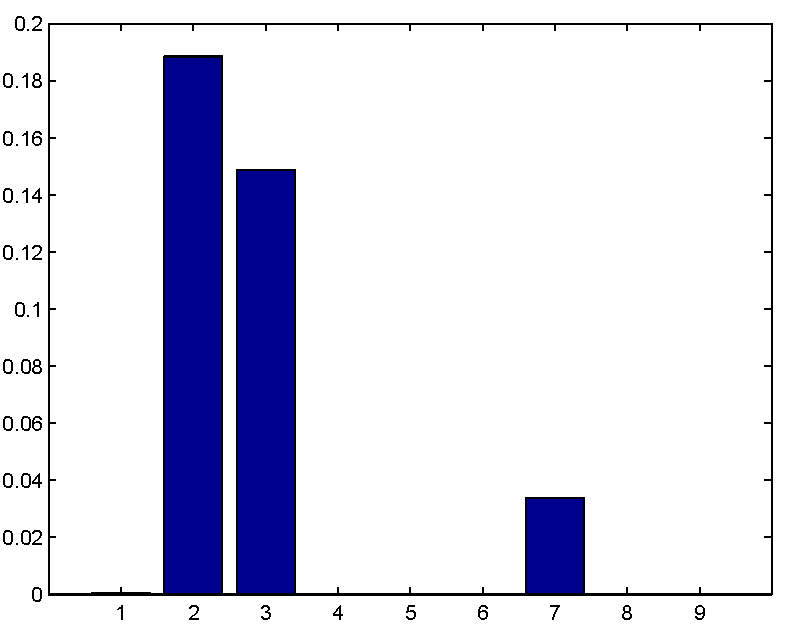
\includegraphics[width=0.4\textwidth]{../diagrams/supplMocapScalesRbf}
	\label{fig:suppMocap1}
}
\subfigure[]{
	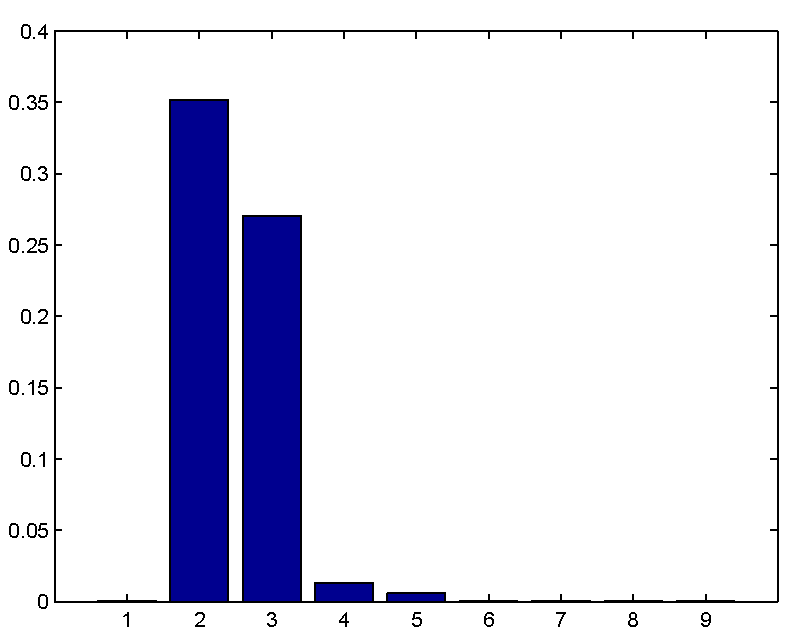
\includegraphics[width=0.4\textwidth]{../diagrams/supplMocapScalesMatern}
	\label{fig:suppMocap2}
}
\end{center}
\caption{\small{
The values of the scales of the ARD kernel after training on the motion capture dataset using the RBF (fig: \subref{fig:suppMocap1}) and the Mat\'ern (fig: \subref{fig:suppMocap2}) covariance function to model the dynamics for VGPDS. The scales that have zero value ``switch off'' the corresponding dimension of the latent space. The latent space is, therefore, 3-D for \subref{fig:suppMocap1} and 4-D for \subref{fig:suppMocap2}. Note that the scales were initialized with very similar values.
}
}
\label{fig:supplMocap1}
\end{figure}


\begin{figure}[ht]
\begin{center}
\subfigure[]{
	%\includegraphics[width=0.48\textwidth]{../diagrams/supplMocapBody23GpdsRbf}
	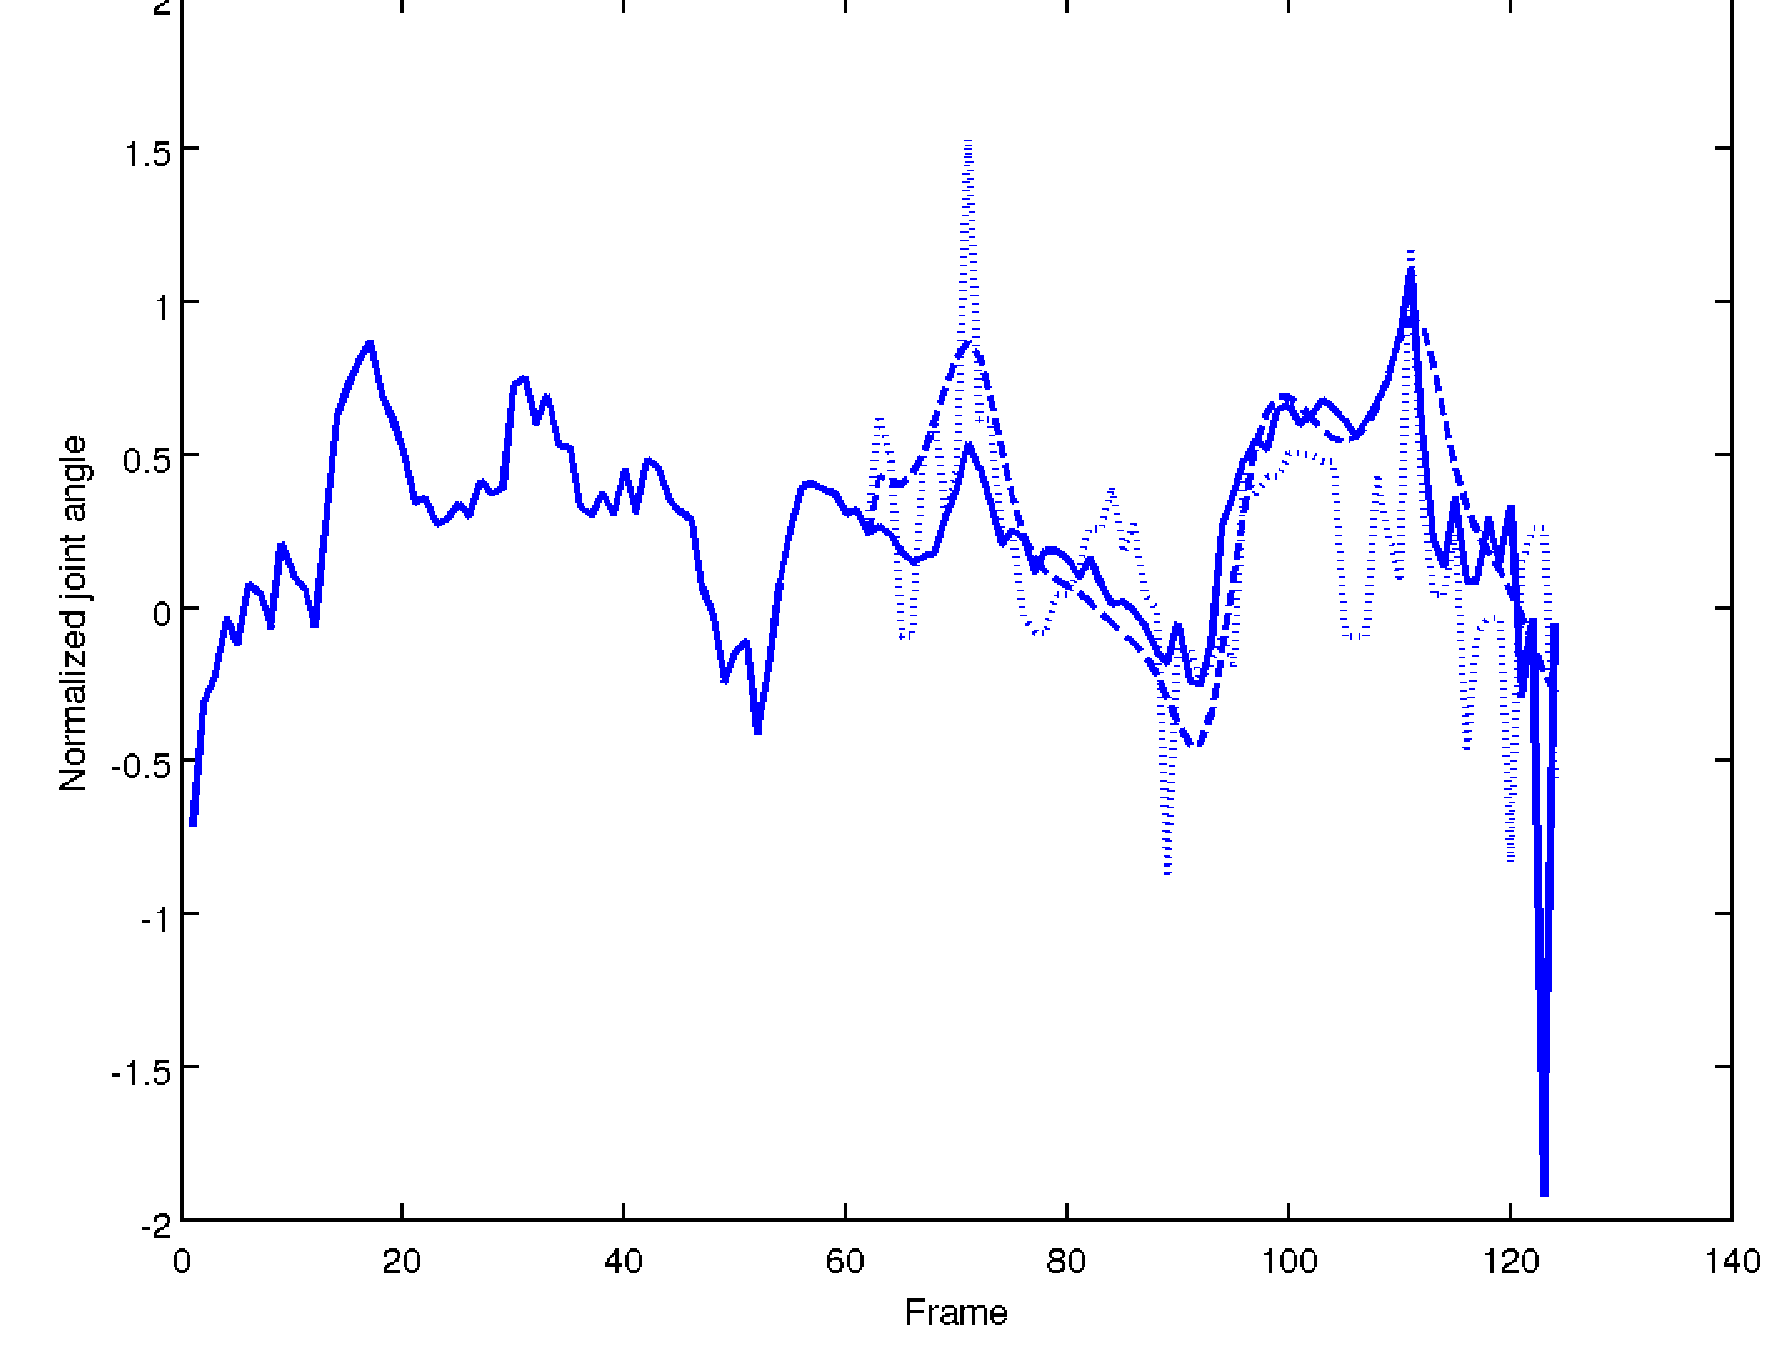
\includegraphics[width=0.48\textwidth]{../diagrams/supplMocapBody28GpdsMatern}
	\label{fig:suppMocap3}
}
\subfigure[]{
	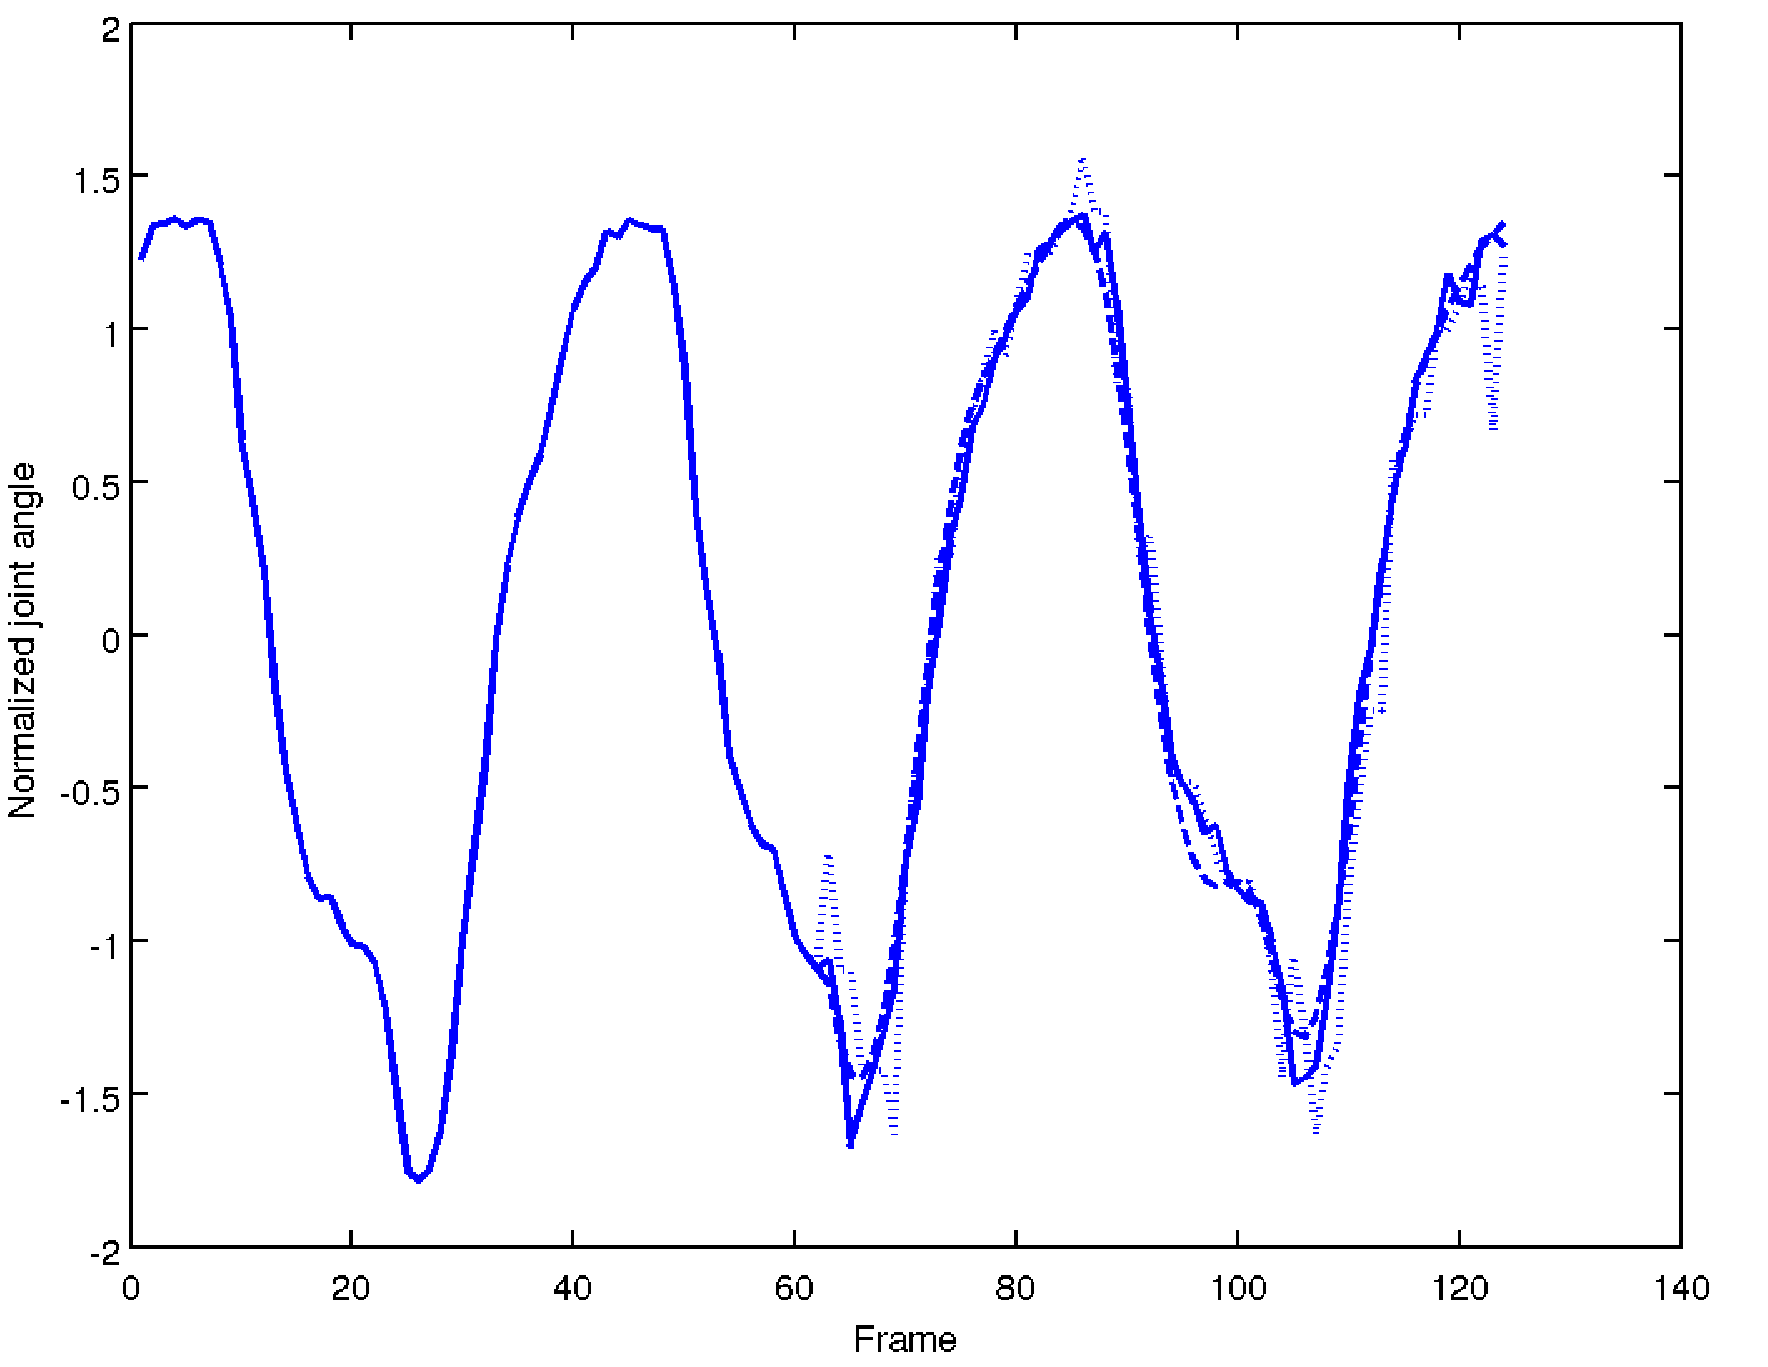
\includegraphics[width=0.48\textwidth]{../diagrams/supplMocapLeg5GpdsMatern}
	\label{fig:suppMocap4}
}
\end{center}
\caption{\small{
The prediction for two of the test angles for the body (fig: \ref{fig:suppMocap3}) and for the legs part (fig: \ref{fig:suppMocap3}). Continuous line is the original test data, dotted line is nearest neighbour in scaled space, dashed line is VGPDS (using the RBF covariance function for the body reconstruction and the Mat\'ern for the legs).
}
}
\label{fig:supplMocap2}
\end{figure}




\begin{figure}[ht]
\begin{center}
\subfigure[]{
	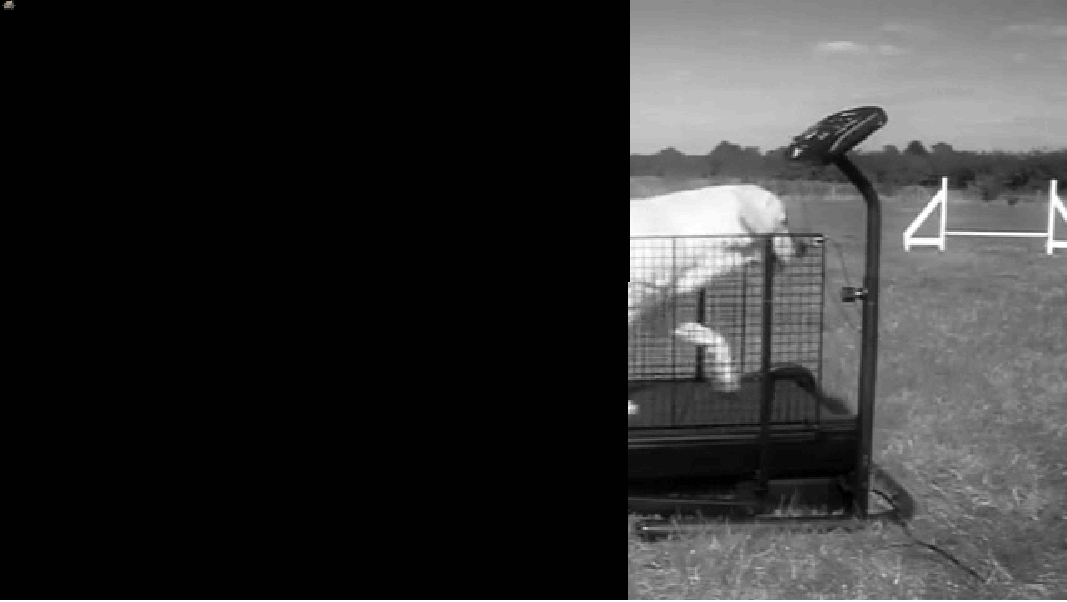
\includegraphics[width=0.23\textwidth]{../diagrams/supplDogPredYts5}
	\label{fig:suppDog1}
}
\subfigure[]{
	\includegraphics[width=0.23\textwidth]{../diagrams/supplDogPredGpds5}
	\label{fig:suppDog2}
}
\subfigure[]{
	\includegraphics[width=0.23\textwidth]{../diagrams/supplDogPredYts6}
	\label{fig:suppDog3}
}
\subfigure[]{
	\includegraphics[width=0.23\textwidth]{../diagrams/supplDogPredGpds6}
	\label{fig:suppDog4}
}
\end{center}
\caption{\small{
 Some more examples for the reconstruction achieved for the `dog' dataset. $40\%$ of the test image's pixels (figures \subref{fig:suppDog1} and \subref{fig:suppDog3}) were presented  to the model, which was able to successfully reconstruct them, as can be seen in \subref{fig:suppDog2} and \subref{fig:suppDog4}.
}
}
\label{fig:supplDog}
\end{figure}



\end{document}
